%%%%%%%%%%%%%%%%%%%%%%% file template.tex %%%%%%%%%%%%%%%%%%%%%%%%%
%
% This is a general template file for the LaTeX package SVJour3
% for Springer journals.          Springer Heidelberg 2010/09/16
%
% Copy it to a new file with a new name and use it as the basis
% for your article. Delete % signs as needed.
%
% This template includes a few options for different layouts and
% content for various journals. Please consult a previous issue of
% your journal as needed.
%
%%%%%%%%%%%%%%%%%%%%%%%%%%%%%%%%%%%%%%%%%%%%%%%%%%%%%%%%%%%%%%%%%%%
%
% First comes an example EPS file -- just ignore it and
% proceed on the \documentclass line
% your LaTeX will extract the file if required
\begin{filecontents*}{example.eps}
%!PS-Adobe-3.0 EPSF-3.0
%%BoundingBox: 19 19 221 221
%%CreationDate: Mon Sep 29 1997
%%Creator: programmed by hand (JK)
%%EndComments
gsave
newpath
  20 20 moveto
  20 220 lineto
  220 220 lineto
  220 20 lineto
closepath
2 setlinewidth
gsave
  .4 setgray fill
grestore
stroke
grestore
\end{filecontents*}
%
\RequirePackage{fix-cm}
%
%\documentclass{svjour3}                     % onecolumn (standard format)
%\documentclass[smallcondensed]{svjour3}     % onecolumn (ditto)
%\documentclass[smallextended]{svjour3}       % onecolumn (second format)
\documentclass[twocolumn]{svjour3}          % twocolumn
%
\smartqed  % flush right qed marks, e.g. at end of proof
%
\usepackage{graphicx}
\usepackage{multirow}
\usepackage{xcolor}             % Sylli,
\usepackage{amsmath,amsfonts}   % Sylli,
\usepackage{amssymb}            % Sylli,
\usepackage{dsfont}             % Sylli,
\usepackage{microtype}          % Sylli,
\usepackage{array}              % Sylli,
\usepackage{enumitem}           % Sylli, to add parameters to the list
\usepackage{makecell}           % Sylli, for the table
\usepackage{colortbl}           % Sylli, for the colors of the table

% Sylli, defined custom colors for the table
\definecolor{Gray}{gray}{0.8}
\definecolor{lGray}{gray}{0.9}
\definecolor{featurebased}{rgb}{0.57, 0.66, 0.77}
\definecolor{rocket}{rgb}{0.78,0.15,0.95}
\definecolor{convbased}{rgb}{0.34, 0.59, 0.97}
\definecolor{transbased}{rgb}{0.95,0.71, 0.28}

% \usepackage{mathptmx}      % use Times fonts if available on your TeX system
%
% insert here the call for the packages your document requires
%\usepackage{latexsym}
% etc.
%
% please place your own definitions here and don't use \def but
% \newcommand{}{}
\newcommand{\journalv}[1]{{\color{red} #1}\normalcolor} % Sylli, for the journal version
%
% Insert the name of "your journal" with
% \journalname{myjournal}
%
\begin{document}

\title{MSAD: A Deep Dive into Model Selection for Time series Anomaly Detection
%\thanks{Grants or other notes about the article that should go on the front page should be placed here. General acknowledgments should be placed at the end of the article.}
}
% \subtitle{Extending Model Selection for Anomaly Detection (MSAD-E) in Time Series with Weighted Averages}

\titlerunning{MSAD-E}        % if too long for running head

\author{
Emmanouil Sylligardos \and
John Paparrizos \and
Themis Palpanas \and
Pierre Senellart \and
Paul Boniol
}

% \authorrunning{Short form of author list} % if too long for running head

\institute{
    E. Sylligardos \at
    École Normale Supérieure, Paris, France \\
    % Tel.: +123-45-678910\\
    % Fax: +123-45-678910\\
    \email{emmanouil.sylligardos@ens.fr}           %  \\
    % \emph{Present address:} of F. Author  %  if needed
    % \and
    % J. Paparrizos \at
    % \email{test@gmail.com}
    % \and
    % T. Palpanas \at
    % \email{themis@mi.parisdescartes.fr}
    % \and
    % P. Senellart \at
    % \email{test@gmail.com}
    % \and
    % P. Boniol \at
    % \email{paul.boniol@inria.fr}
}

\date{Received: date / Accepted: date}
% The correct dates will be entered by the editor


\maketitle

\begin{abstract}
Time series have seen a rapidly growing interest throughout the last two decades. The research community has thus been focusing on providing tools in multiple domains of time series analysis. The main domains are a) clustering, b) pattern recognition, c) anomaly detection, etc. In anomaly detection, multiple algorithms have been proposed, however research and benchmarks point out that none of the proposed anomaly detectors can succeed in all the different fields where time series are used (medicine, industry, etc.). To this end, model selection approaches have been proposed that combine the multiple anomaly detectors to achieve greater, inter-domain results. In this work, we will build on top of MSAD, a model selection framework for anomaly detection in time series. MSAD was proposed so that it reads a time series and simply predicts a single detector to use on this time series. We will provide MSAD the ability to predict multiple detectors, each one of them with a different weight, and then combine these detectors according to the aforesaid weights. We hope that this approach, namely MSAD-E, provides even better results and anomaly detection power than before.
\keywords{Time Series \and Anomaly Detection \and Model Selection \and Machine Learning}
% \PACS{PACS code1 \and PACS code2 \and more}
% \subclass{MSC code1 \and MSC code2 \and more}
\end{abstract}


% ------ Content ------

\section{Introduction}

\begin{figure}
    \centering
    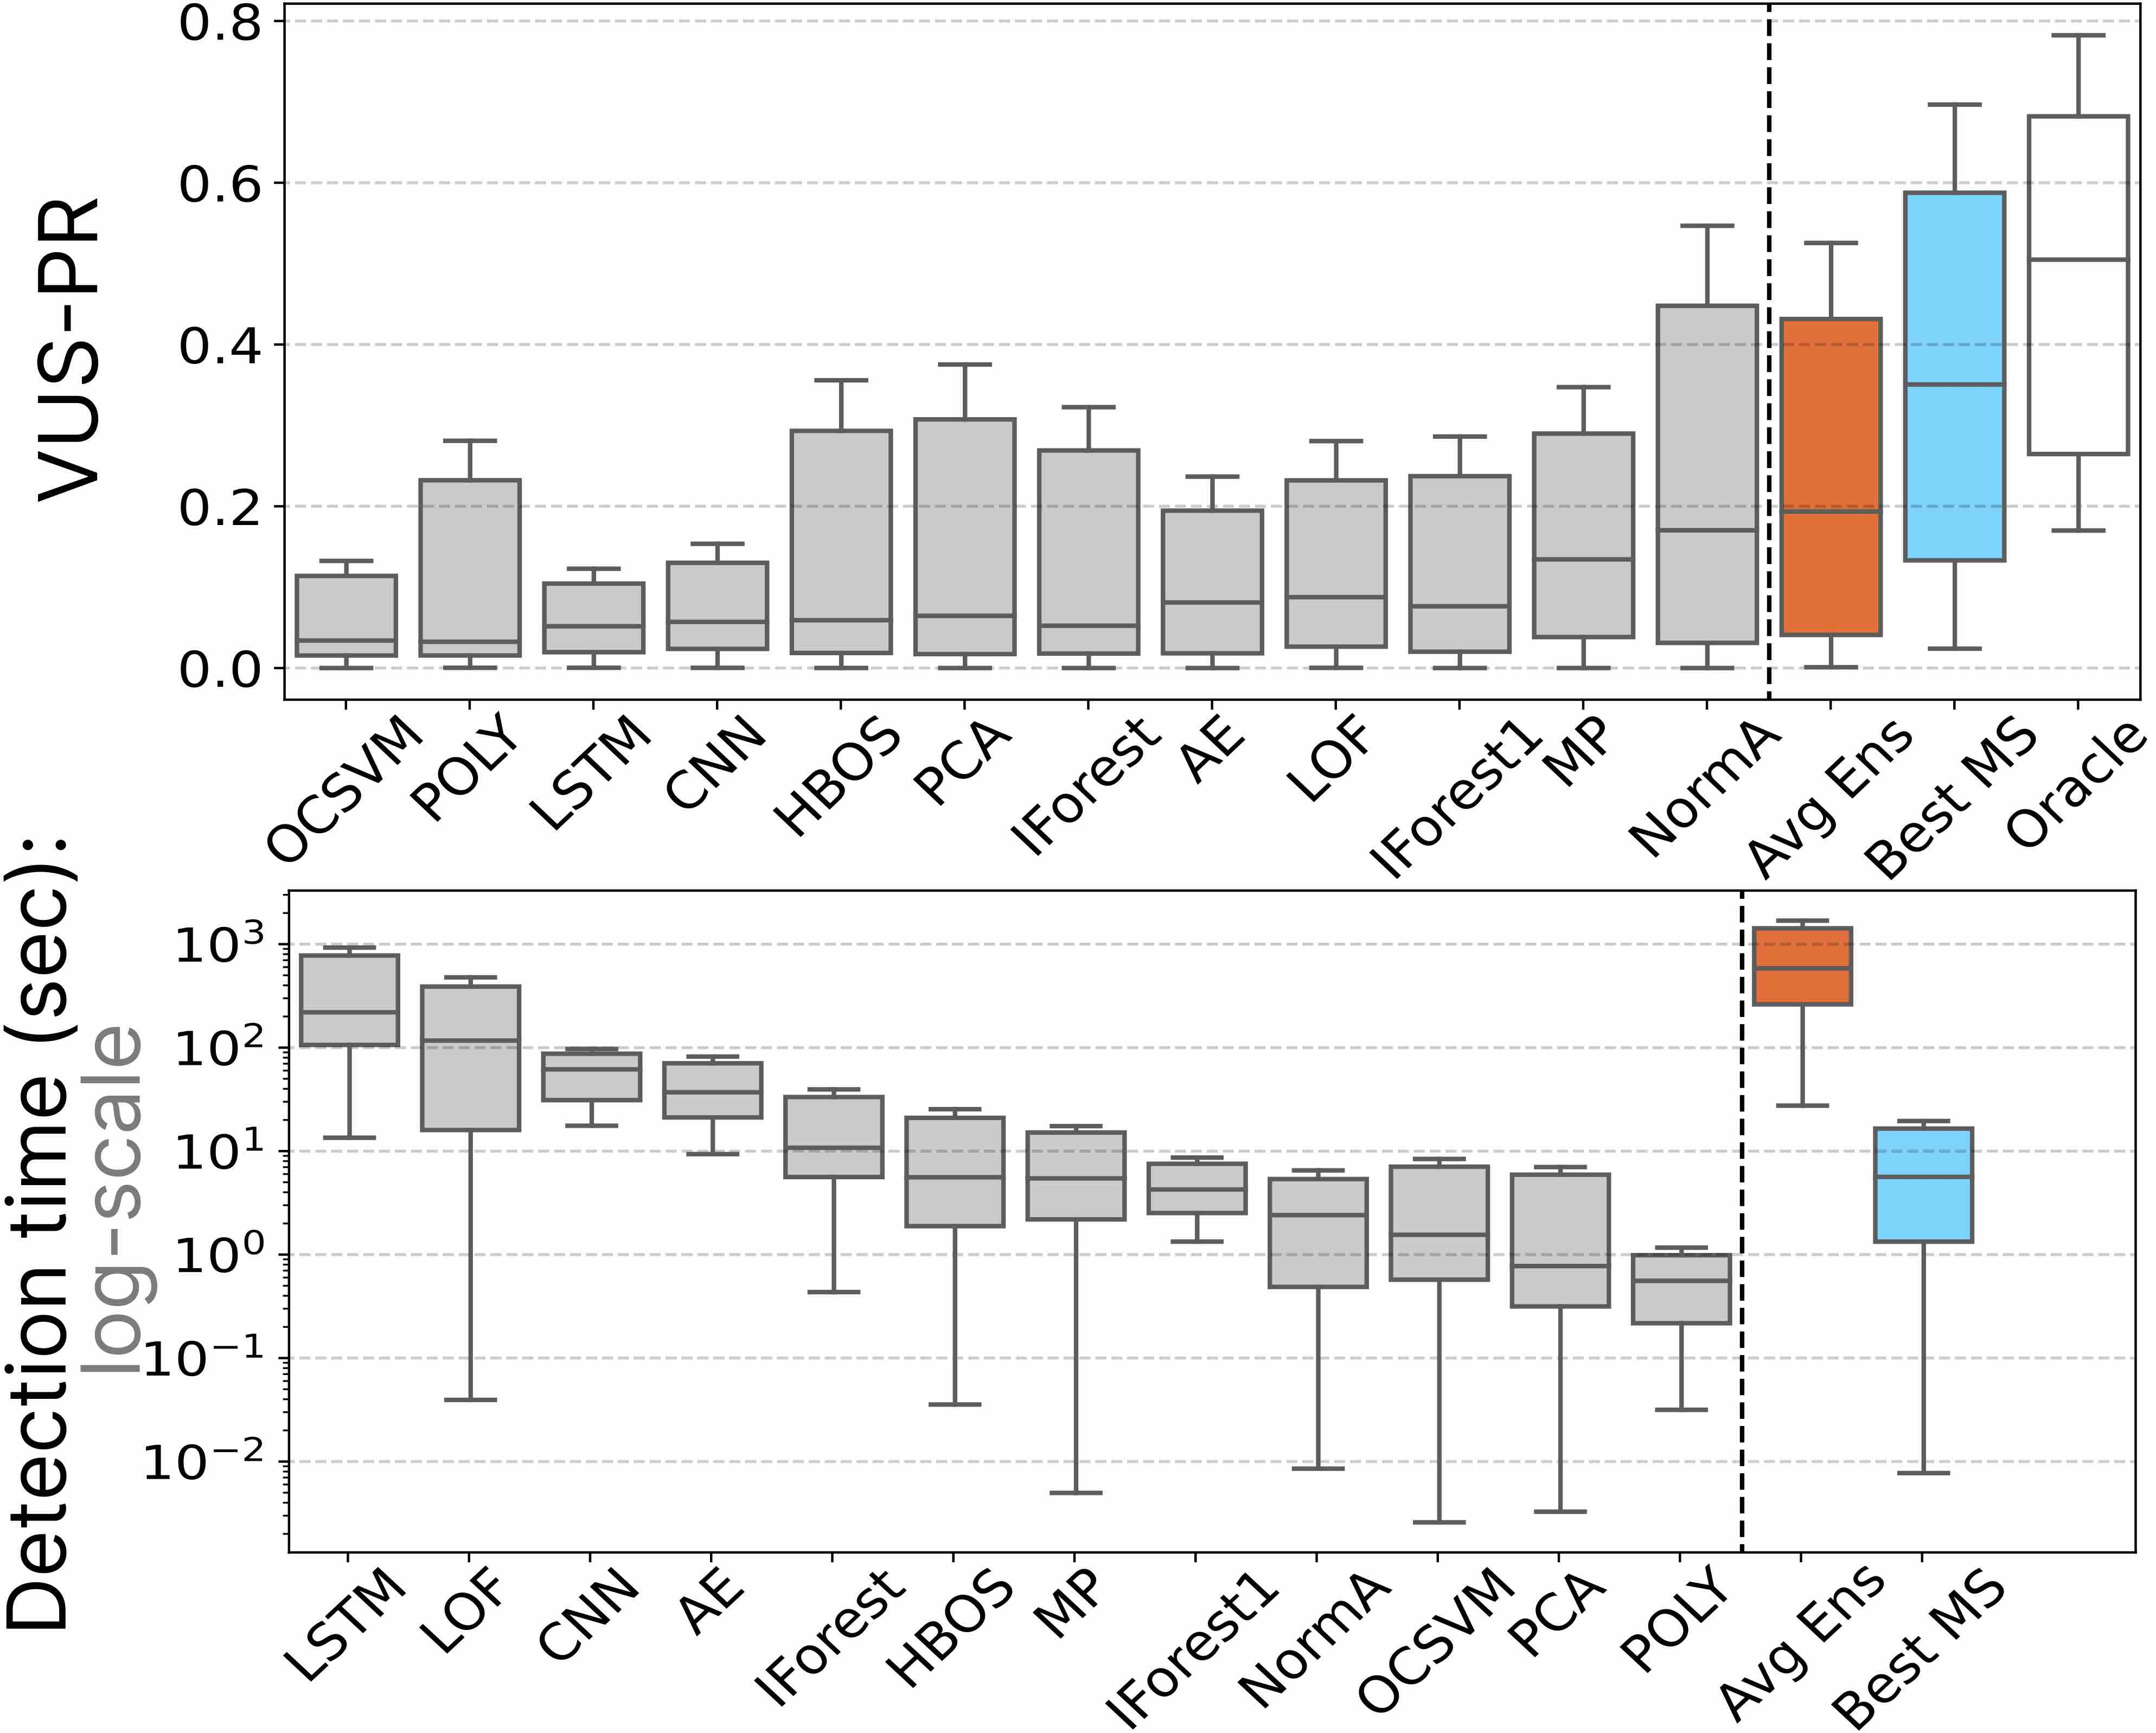
\includegraphics[width=1\linewidth]{figures/Fig1.jpg}
    \caption{Summary of our evaluation on the TSB-UAD benchmark~\cite{10.14778/3529337.3529354} of model selection methods (best in blue) when compared to 12 anomaly detection methods and the Avg Ens (in orange).}
    \label{fig:intro_fig}
\end{figure}

% TODO: Fix references
Extensive collections of time-dependent measurements are a reality in every scientific domain~\cite{Palpanas2015,DBLP:journals/dagstuhl-reports/BagnallCPZ19,Palpanas2019,paparrizos2021vergedb,liu2023amir,paparrizos2018fastthesis}. The recording of these measurements results in an ordered sequence of real-valued data points, commonly referred to as {\em time series}~\cite{paparrizos2015k,paparrizos2017fast,bariya2021k,paparrizos2022fast,paparrizos2023accelerating}. Analyzing time series data is becoming increasingly important in virtually every scientific and industrial domain~\cite{DBLP:conf/edbt/EchihabiZP21,DBLP:journals/pvldb/EchihabiPZ21,liu2021decomposed,jiang2020pids,jiang2021good,dziedzic2019band,paparrizos2019grail,paparrizos2020debunking,paparrizos2016detecting,paparrizos2016screening,mckeown2016predicting,goel2016social,DBLP:journals/pvldb/0003WNP22,DBLP:conf/eenergy/PetraliaCBP23}\journalv{, including astronomy~\cite{huijse2014computational}, biology~\cite{bar2003continuous}, economics~\cite{lutkepohl2004applied}, energy sciences~\cite{bach2017flexible}, engineering~\cite{uehara2002extraction}, environmental sciences~\cite{goddard2003geospatial}, medicine~\cite{richman2000physiological}, neuroscience~\cite{biswal2010toward}, and social sciences~\cite{brockwell2016introduction}.} Anomaly detection, in particular, has received ample academic and industrial attention~\cite{page1957problems,fox1972outliers}\journalv{, and has become a significant problem that finds} applications across a wide range of domains and situations. These applications share the same goal~\cite{statisticaloutliers,DBLP:conf/vldb/SubramaniamPPKG06,DBLP:conf/icdm/YehZUBDDSMK16}: analyzing time series to identify observations that do not correspond to an expected behavior inferred from previously observed data. In practice, anomalies can correspond to~\cite{aggarwal2017introduction}: (i) noise or erroneous data (e.g., broken sensors); or (ii) actual data of interest (e.g., abnormal behavior of the observed system). In both cases, detecting such types is crucial for many applications~\cite{IMSGroundtruth,DBLP:conf/healthcom/HadjemNK16}.

In recent years, many techniques have been proposed for time-series anomaly detection. Multiple surveys and benchmarks summarize and analyze the state-of-the-art proposed methods~\cite{blazquez2021review,10.14778/3529337.3529354,10.14778/3538598.3538602,10.14778/3551793.3551830,10.14778/3476249.3476307,wu2020current,7424283,jacob2020exathlon,Kim2021TowardsAR}. Such surveys and benchmarks provide a holistic view of anomaly detection methods and how they perform. Unfortunately, these benchmark and evaluation studies demonstrated that no overall best anomaly detection methods exist when applied to very heterogeneous time series (i.e., coming from very different domains). In practice, we observe that some methods outperform others on specific time series with either specific characteristics (e.g., stationary or non-stationary time series) or anomalies (e.g., point-based or sequence-based anomalies). 

To overcome the above limitation, ensembling solutions have been proposed~\cite{10.1145/2830544.2830549} that consist of running all existing anomaly detection methods and averaging all anomaly scores. Figure~\ref{fig:intro_fig} shows that this solution (in orange) is outperforming all individual existing techniques in the TSB-UAD benchmark~\cite{10.14778/3529337.3529354,boniol2022theseus}. Nevertheless, as shown in Figure~\ref{fig:intro_fig}, such solutions require running all methods, resulting in an excessive cost that is not feasible in practice.

Therefore, the only scalable and viable solution for solving anomaly detection over very different time series collected from various domains is to propose a model selection method that will select, based on time series characteristics, the best anomaly detection method to run. This topic has been tackled in several recent research works related to AutoML (Automated Machine Learning) for the general case of anomaly detection~\cite{NEURIPS2021_23c89427,ying2020automated} \journalv{and also for time series~\cite{https://doi.org/10.48550/arxiv.2009.04395,https://doi.org/10.48550/arxiv.2210.01078}}. Nevertheless, existing AutoML solutions require (i) a universal objective function among models, which is not applicable to anomaly detection methods; (ii) a predefined set of features, which is difficult to obtain for time series due to varying lengths and the lack of standardized featurization solutions; (iii) running multiple anomaly detection methods several times, which is prohibitively expensive in practice; or (iv) labeled anomalies, which (in contrast to classification tasks) are difficult to obtain. Therefore, more work is needed in order to render AutoML solutions applicable to time-series anomaly detection. 

The objective is to train a time series classification model on time series for which we know in advance which anomaly detection method is the best. However, the lack of a benchmark with labeled time series has been a limiting factor for training robust model selection models (this only changed very recently~\cite{10.14778/3529337.3529354,10.14778/3538598.3538602,kdd21}). Therefore, there exists no experimental evaluation that measures the effectiveness of classification methods for the task of model selection for time series anomaly detection. Though, such an evaluation is very important for determining which time series classification methods are accurate as model selection methods, and which solutions should be considered in unsupervised settings (i.e., using model selection approaches on time series from domains that were not included in the training set). These results would help the design and effectiveness of general AutoML pipelines for time series.

Thus, in this paper, we evaluate the performance of time series classification methods used as model selection for anomaly detection in time series. To do so, we propose a pipeline that enables any kind of time series classifier to be used for any univariate time series with different lengths. We then compare the execution time and accuracy for feature-based, traditional time series classifiers and deep learning classification algorithms. We also measure how these models perform when trained on time series of a given domain (e.g., electrocardiogram~\cite{Moody}) and tested on time series from a different domain (e.g., robotics sensors measurements~\cite{5573462}). 

Overall, we compare 16 different classifiers over 1980 time series and 12 anomaly detection methods from the recent anomaly detection benchmark TSB-UAD. Thus, we propose the first extensive experimental evaluation of time series classification as model selection for anomaly detection. Our results demonstrate that model selection methods outperform every single anomaly detection method while being in the same order of magnitude regarding execution time. Figure~\ref{fig:intro_fig} shows a summary of our experimental evaluation, where the best model selection method (in blue in Figure~\ref{fig:intro_fig}) is up to 2.8$\times$ more accurate than the best anomaly detection method in the TSB-UAD benchmark and 1.9$\times$ more accurate than the ensembling solution mentioned above. This evaluation is the first step to demonstrate the accuracy and efficiency of time series classification algorithms for anomaly detection. It represents a strong baseline that can then be used to guide the choice of approaches for the model selection step in more general AutoML pipelines.\journalv{Overall, the paper is organized as follows.}

\journalv{We start with a detailed discussion of the relevant background and related work for anomaly detection in time series (Section~\ref{sec:background}). Then, we present our contributions:}
\begin{itemize}%[noitemsep, topsep=0pt, parsep=0pt, partopsep=0pt, leftmargin=0.4cm]
	\item We cast the model selection problem for time-series anomaly detection methods into a time-series classification problem. We describe and study the need to evaluate time series classification methods for model selection (Section~\ref{sec:problem_def}). 
	\item We introduce our novel pipeline for model selection applied to anomaly detection in time series. As this pipeline is generic, we describe how it can be used with both feature-based classification methods, traditional time series classification methods, and deep learning-based methods (Section~\ref{sec:proposed}).
	\item We describe our experimental framework (on top of the recent anomaly detection benchmark TSB-UAD~\cite{10.14778/3529337.3529354}), and provide details on both anomaly detection methods and time series classification methods considered in this paper (Section~\ref{sec:exp}). We make all our material publicly available online~\cite{ourcode} and provide an interactive \journalv{Web application}~\cite{ourwebsite} for exploring our results. 
	\item We present an extensive experimental evaluation, measuring the anomaly detection accuracy and execution time (both training and inference) of model selection algorithms (Section~\ref{exp:overalleval}). We evaluate the influence of important parameters and the relationship between classification and anomaly detection accuracy (Sections~\ref{exp:windowlength}, \ref{exp:datasets}, and \ref{exp:detectionvsclass}). Moreover, we measure the transferability of model selection algorithms to new types of time series by testing multiple combinations of train and test datasets that do not contain the same kinds of time series (Section~\ref{exp:sup2unsup}).
\end{itemize}
Finally, we conclude with the implications of our work and discuss possible future directions that could help improve both the accuracy and the execution time of our proposed pipeline (Section~\ref{sec:conclusions}).
\section{Background and Related Work}
\label{sec:background}

We first introduce \journalv{formal} notations useful for the rest of the paper (Section~\ref{sec:notation}). Then, we review \journalv{in detail} existing time-series anomaly detection methods (Section~\ref{sec:ad_methods}), and discuss their limitations when applied to large heterogeneous sets of time series (Section~\ref{sec:limitation}). 

\subsection{Time-Series and Anomaly Score Notations}
\label{sec:notation}

\journalv{In this section, we review notations for time series and anomaly score sequences.}

\textbf{Time Series: }A time series $T \in \mathbb{R}^n $ is a sequence of real-valued numbers $T_i\in\mathbb{R}$ $[T_1,T_2,...,T_n]$, where $n=|T|$ is the length of $T$, and $T_i$ is the $i^{th}$ point of $T$. We are typically interested in local regions of the time series, known as subsequences. A subsequence $T_{i,\ell} \in \mathbb{R}^\ell$ of a time series $T$ is a continuous subset of the values of $T$ of length $\ell$ starting at position $i$. Formally, $T_{i,\ell} = [T_i, T_{i+1},...,T_{i+\ell-1}]$. \journalv{We then define a} dataset $\mathcal{D}$, which is a set of time series. Note that the time series contained in $\mathcal{D}$ can be of diverse lengths. We define the size of $\mathcal{D}$ as $|\mathcal{D}|$.

\textbf{Anomaly Score Sequence: }For a time series $T \in \mathbb{R}^n $, an anomaly detection method (or detector) $D$ returns an anomaly score sequence $S_T$. For point-based approaches (i.e., methods that return a score for each point), we have $S_T \in \mathbb{R}^n$. For subsequence-based approaches (i.e., methods that return a score for each subsequence of a given length $\ell$), we have $S_T \in \mathbb{R}^{n-\ell}$ and $S_T = [{S_T}_1,{S_T}_2,...,{S_T}_{n-\ell}]$ with ${S_T}_i \in [0,1]$. In most applications, the anomaly score has to be the same length as the time series. \journalv{Thus, for subsequence-based approaches, we define:
\begin{equation*}
    \begin{aligned}
        S_T =\, &[{S_T}_1]_{i\in[0,\ell/2]}\, + \\
                &[{S_T}_1, {S_T}_2, \ldots, {S_T}_{n-\ell}]\, + \\
                &[{S_T}_{n-\ell}]_{i\in[0,\ell/2]} \text{ with } |S_T| = |T|
    \end{aligned}
\end{equation*}
}

\textbf{Anomaly Detection Accuracy: }For a time series $T \in \mathbb{R}^n $, an anomaly detection method (or detector) $D$ that returns an anomaly score sequence $D(T) = S_T$ and labels $L \in [0,1]^n$ that indicated with 0 or 1 if the points in $T$ are normal or abnormal respectively, we define $Acc:\mathbb{R}^n,\{0,1\}^n \rightarrow [0,1]$ as an accuracy function for which $Acc(D(T),L)$ indicates how $D$ is accurate (i.e., and produce an anomaly score close to 1 when the label is equal to 1) when applied on $T$ and accordingly to $L$. The closer to one, the better.

\begin{figure}
    \centering
    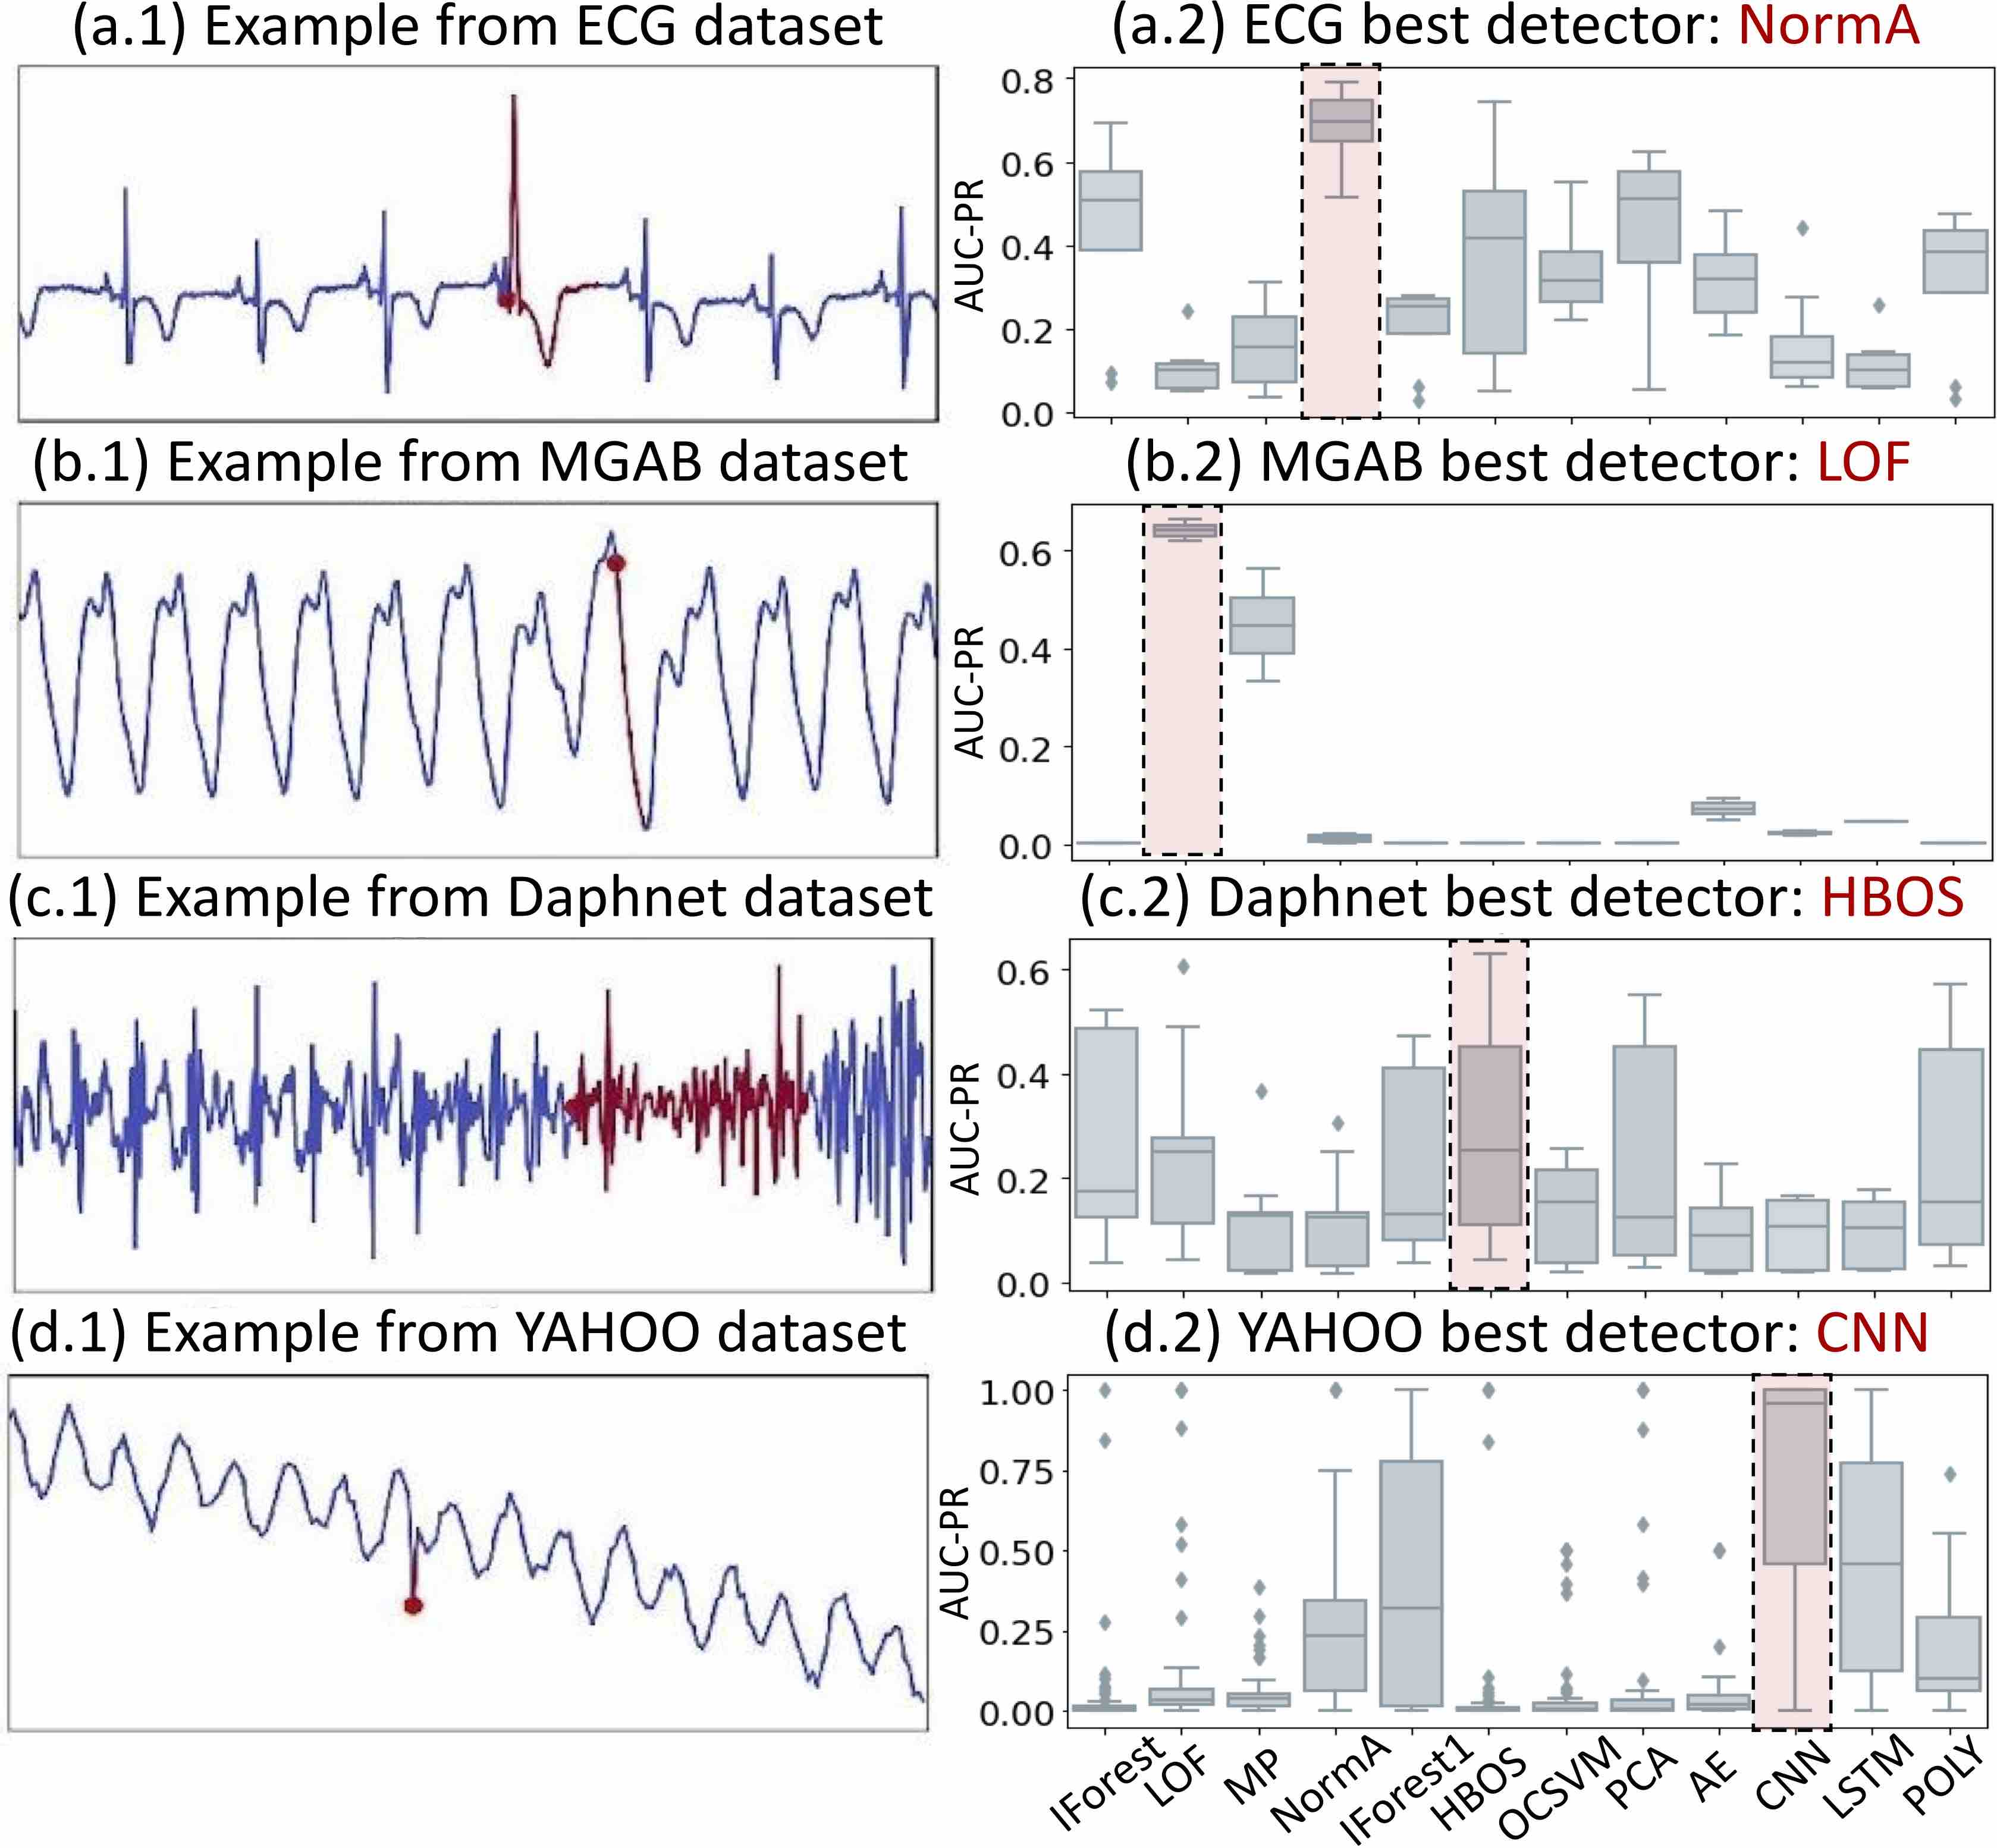
\includegraphics[width=1\linewidth]{figures/Fig2.jpg}
    \caption{Accuracy of 12 anomaly detection methods on 4 datasets.}
    \label{fig:diversity}
\end{figure}

\subsection{Anomaly Detection Methods for Time Series}
\label{sec:ad_methods}

\journalv{Anomaly detection in time series is a crucial task for many relevant applications. Therefore,} several different methods (for diverse types of time series, or applications) have been proposed in the literature. One type of anomaly detection method is \textit{discord-based methods}. These methods focus on the analysis of subsequences for the purpose of detecting anomalies in time series, mainly by utilizing nearest neighbor distances among subsequences \cite{DBLP:conf/icdm/YehZUBDDSMK16,DBLP:conf/edbt/Senin0WOGBCF15,Keogh2007,Liu2009,DBLP:conf/adma/FuLKL06,DBLP:conf/sdm/BuLFKPM07,DBLP:journals/datamine/LinardiZPK20}. 

Instead of measuring nearest neighbor distances, \textit{proximity-based methods} focus on estimating the density of particular types of subsequences in order to either extract a normal behavior or isolate anomalies. Since a subsequence can be seen as a multidimensional point (with the number of dimensions corresponding to the subsequence length), general outlier detection methods can be applied for time series anomaly detection~\cite{liu_isolation_2008,Breunig:2000:LID:342009.335388,ma2020isolation}. Among them, Isolation Forest~\cite{liu_isolation_2008} has been shown to work particularly well for time series anomaly detection task~\cite{Series2GraphPaper}. Moreover, recent proximity-based methods dedicated to identifying abnormal subsequences in time series have been proposed. For instance, NormA, a proximity-based method that first clusters data to obtain the normal behavior~\cite{norm,boniol_unsupervised_2021,DBLP:conf/icde/BoniolLRP20,boniol2021sand,boniol2021sanddemo}, \journalv{or Series2Graph that converts the time series into a graph to facilitate the detection of anomalies~\cite{Series2GraphPaper}, have both demonstrated} strong performance.

Furthermore, \textit{forecasting-based methods}, such as recurrent neural network-based ~\cite{malhotra_long_2015} or convolutional network-based ~\cite{8581424}, have been proposed for this task. Such methods use the past values as input, predict the following one, and use the forecasting error as an anomaly score. Such methods are usually trained on time series without anomalies, or make the assumption that the anomalies are significantly less frequent than the normal behaviors.

Finally, \textit{reconstruction-based methods}, such as autoencoder approaches ~\cite{10.1145/2689746.2689747}, are trained to reconstruct the time series and use the reconstruction error as an anomaly score. As both forecasting and reconstruction-based categories detect anomalies using prediction errors (either forecasting or reconstruction error), we can group them into \textit{prediction-based methods}. 

\subsection{Limitations of Anomaly Detection Methods} % on heterogeneous data}
\label{sec:limitation}

Recent benchmarks and experimental evaluations have been proposed in the literature~\cite{10.14778/3538598.3538602,10.14778/3551793.3551830,kdd21}. Such benchmarks provide a large collection of time series from various domains and evaluate multiple methods belonging to the categories mentioned above. However, these experimental evaluations led to the same conclusion: no method exists that outperforms all the others on all time series from various domains. Figure~\ref{fig:diversity}, which depicts the accuracy of 12 diverse anomaly detection methods\footnote{We use 12 methods that have been employed in previous studies ~\cite{10.14778/3529337.3529354,10.14778/3551793.3551830}. Note that other methods and variations exist that may lead to improved results.} on four time series datasets, illustrates the conclusion above. In Figure~\ref{fig:diversity} (a.2), we observe that NormA is the most accurate model on the ECG dataset~\cite{Moody} (a time series example is depicted in Figure~\ref{fig:diversity} (a.1)). However, Local Outlier Factor (LOF)~\cite{Breunig:2000:LID:342009.335388}, and Matrix profile (MP)~\cite{DBLP:conf/icdm/YehZUBDDSMK16} are significantly outperforming NormA on the MGAB dataset~\cite{markus_thill_2020_3762385} (see Figure~\ref{fig:diversity} (b.2)), whereas CNN~\cite{8581424} is outperforming NormA, LOF, and MP on the YAHOO dataset~\cite{yahoo} (see Figure~\ref{fig:diversity} (d.2)). The following two reasons explain this large difference in performance among datasets.

\subsubsection{\textbf{Heterogeneity in anomaly types}}

First, There are three types of time-series anomalies: \textit{point}, \textit{contextual}, and \textit{collective} anomalies. \textit{Point} anomalies refer to data points that deviate remarkably from the rest of the data. Similarly, \textit{Contextual} anomalies refer to data points within the expected range of the distribution (in contrast to point anomalies) but deviate from the expected data distribution, given a specific context (e.g., a window). For instance, Figure~\ref{fig:diversity} (d.1) illustrates a time series from the YAHOO dataset with a \textit{Contextual} anomaly. The value of the anomalies is inside the range of normal values, but is abnormal in the context of the distribution of values of the surrounding point. For this particular types of anomalies, \textit{reconstruction} and \textit{forcasting}-based methods are particularly accurate (as shown in Figure~\ref{fig:diversity} (d.2))

\textit{Collective} anomalies refer to sequences of points that do not repeat a typical (previously observed) pattern. The first two categories, namely, point and contextual anomalies, are referred to as \textit{point-based} anomalies, whereas \textit{collective} anomalies are referred to as \textit{subsequence} anomalies. For instance, Figure~\ref{fig:diversity} (a.1), (b.1), and (c.1) show three time series with sequence anomalies. However, even for time series belonging to the same anomaly type categories, we observe that the most accurate models are all different.  

\subsubsection{\textbf{Heterogeneity in time series structures}}

This diversity in model accuracy can be explained by other factors related to the time series structures. Indeed, on top of these categories mentioned above, the combination of them also matters. First, we need to differentiate time series containing \textit{single} anomalies from time series containing \textit{multiple} anomalies. Last, the \textit{multiple} time series category has to be divided into two subcategories, namely time series containing \textit{multiple different} and \textit{multiple similar} anomalies. For instance, methods based on neighbor distance computation such as LOF are very accurate in detecting \textit{single} or \textit{multiple different} anomalies, but less accurate for \textit{multiple similar}. To illustrate this point, Figure~\ref{fig:diversity} (a.2) depicts the results of 12 anomaly detection methods on the ECG dataset (that contains \journalv{a large number of} \textit{multiple similar} anomalies), for which LOF accuracy is low. On the contrary, Figure~\ref{fig:diversity} (b.2) depicts the results of the same 12 anomaly detection methods on the MGAB dataset (that contains \textit{multiple different} anomalies), for which LOF accuracy is high.

On top of the large variety of time series and anomaly characteristics mentioned above, time series can have distinct statistical characteristics, resulting in an even larger variability in the accuracy of anomaly detection methods. %To all these differences between time series, resulting in large variability in the accuracy of anomaly detection methods, we can add differences in the time series statistical characteristics.
The latter can be the differences between \textit{stationary} (i.e., with a constant distribution of values over time) and \textit{non-stationary} (i.e., with a changing distribution of values over time) time series, or \textit{single normality} (i.e., time series containing only one normal behavior) and \textit{multiple normalities} (i.e., time series containing multiple normal behaviors) time series. 
\section{Motivation and Problem}
\label{sec:problem_def}

In this section, we describe solutions that can be applied to solve the limitations mentioned above, and we motivate the benefits of these solutions. We finally formally define the problem.

\subsection{Ensembling Detectors}

The first solution is to ensemble the anomaly scores produced by all the detectors. Multiple ensembling techniques have been proposed in the literature~\cite{10.1145/2830544.2830549} from which \journalv{three} main methods arise: (i) \textit{Averaging}: the average of the anomaly scores for each timestamp, (ii) \textit{Maximizing}: the maximum anomaly score for each timestamp (iii) \textit{Average of Maximum}: the average of the maximum for a randomly selected subset of detectors. \textit{Averaging} strategy is proven to be the more robust and low-risk strategy compared to the other two~\cite{10.1145/2830544.2830549}. Formally, the \textit{Averaging} strategy is defined as follows:

\begin{definition}
    Given time series $T$ of length $n$ and a set of detectors $\mathcal{B}$, \textit{Averaging} strategy is defined as $Avg~Ens = [Avg_1,Avg_2, ..., Avg_m]$ with $Avg_i$ (for $i \in [i,m]$) equals to $Avg_i= (1/|\mathcal{B}|)\sum_{D \in \mathcal{B}} D(T)_i$.
\end{definition}


In the rest of the paper, we call the \textit{Averaging} strategy \textit{Averaging Ensemble (Avg Ens)}. As depicted in Figure~\ref{fig:intro_fig} (a), which shows the accuracy of detectors (in grey) and the Averaging Ensemble (in orange), we observe that such a strategy already outperforms all existing approaches. Nonetheless, such a method requires running all detectors to produce one ensembled anomaly score, resulting in a costly execution time (see Figure~\ref{fig:intro_fig} (b)). In a scenario with very long time series and an increasing number of detectors to consider, such an approach is not sustainable and feasible in practice.

\subsection{Model Selection}

A solution to tackle the limitations mentioned above is to apply model selection based on the characteristics of the time series. The main idea is to train a model to automatically select the best detector (anomaly detection method) for a given time series. In such a case, the user only has to run one model, drastically limiting the execution time required. This topic has been tackled in several recent papers related to AutoML (Automatic Machine Learning). Recent approaches, such as MetaOD~\cite{NEURIPS2021_23c89427,https://doi.org/10.48550/arxiv.2009.04395}, explored meta-learning to identify the best outlier detection algorithm on tabular datasets. 
%Recent studies have also been proposed for the specific case of time series~\cite{https://doi.org/10.48550/arxiv.2009.04395,https://doi.org/10.48550/arxiv.2102.05740}. 
These research works rely on pre-computed models' performances on a subset of datasets to learn a mapping from the dataset's characteristics to the detectors' performance. Methods have been proposed to select models in an unsupervised way~\cite{https://doi.org/10.48550/arxiv.2210.01078}, but require running multiple models in advance, which (like Averaging Ensemble) limit the applicability due to high cost. \journalv{Overall, existing AutoML solutions require: (i) a universal objective function among models, which is not applicable to anomaly detection methods; (ii) a predefined set of features, which is difficult to obtain for time series due to varying lengths and the lack of standardized featurization solutions; and (iii) running multiple anomaly detection methods several times, which is prohibitively expensive in practice.}

\subsection{Classification for Model Selection}

In general, for the specific case of time series, most of the work described above and future AutoML methods will rely on time series classification methods for the model selection step. In such a case, the method aims to classify time series into classes corresponding to the available anomaly detection methods. One time series must be classified into the detector class that maximizes anomaly detection accuracy. However, no existing guidelines indicate which time series classification approach can be used as model selection. Thus, there is a need to evaluate and measure the benefit that time series classification approaches can bring to the anomaly detection task.

The first step is to evaluate the potential gain in accuracy that model selection could bring. To do this, recent time series anomaly benchmarks~\cite{10.14778/3529337.3529354,10.14778/3538598.3538602} can be used. We can evaluate the accuracy upper bound that model selection methods reach on such benchmarks. Thus, we define a hypothetical model called $Oracle$, which, for a given time series, always selects the correct anomaly detector to use (i.e., the most accurate). Formally, $Oracle$ is defined as follows:

\begin{definition}
Given a dataset $\mathcal{D}$ composed of time series $T$ and labels $L$ (with the length of the time series $|T|=n$ non-constant for all time series in $\mathcal{D}$), and a set of detectors $\mathcal{B} = \{D_1, D_i, ..., D_m\}$ with the number of detectors defined as $|\mathcal{B}|=m$, $Oracle(T)= \operatorname*{argmax}_{D \in \mathcal{B}} \big\{Acc\big(D(T),L\big)\big\}$ 
\end{definition}

In the rest of the paper, we call $Oracle$, the hypothetical model $Oracle(T)$ applied to all $T$ in a given benchmark. For example, figure~\ref{fig:intro_fig} shows in white the accuracy of $Oracle$ applied to the TSB-UAD benchmark~\cite{10.14778/3529337.3529354} and demonstrates that a perfect model selection method outperforms the best detector in TSB-UAD and the Averaging Ensemble by a factor of 2.5. This large improvement in accuracy and execution time confirms the potential benefits of model selection applied for time series anomaly detection. Thus, there is a need to evaluate the performances of existing time series classification methods when used as model selection algorithms and how close such methods can get to the $Oracle$.

\subsection{Problem Formulation}

Therefore, based on the limitations and the motivation listed above, we can formalize the problem of model selection as follows:

\begin{problem}
    \label{prob:probdef}
    Given a dataset $\mathcal{D}$ composed of time series $T$ (with the length of the time series $|T|=n$ non-constant for all time series in $\mathcal{D}$) and a set of detectors $\mathcal{B} = \{D_1, D_2, ..., D_m\}$ with the number of detectors defined as $|\mathcal{B}|=m$, we want to build a model selection method $\mathcal{M}$ that takes a time series $T\in \mathcal{D}$ and returns a detector $D\in \mathcal{B}$ (formally $\mathcal{M}: \mathcal{D} \rightarrow \mathcal{B}$) such that, for a given time series $T$ and corresponding label $L$:
    \begin{align*}
        \mathcal{M}(T) = Oracle(T)= \operatorname*{argmax}_{D \in \mathcal{B}} \bigg\{Acc\big(D(T),L\big)\bigg\}
    \end{align*}
\end{problem}
\journalv{In practice, we do not have the label $L$. Therefore, the objective is to build a model $\mathcal{M}$ that estimate the equation above.}

Moreover, as the input of the model $\mathcal{M}$ is a time series (of variable length) and the output is a detector $D$ among a finite number of detectors $\mathcal{B}$, the problem can be seen as a time series classification problem for which the classes are the detectors in $\mathcal{B}$. Therefore, the only requirement is to have computed all $Acc(D(T),L)$ for all $T\in \mathcal{D}$ and all $D\in \mathcal{B}$ and use it as a training set.

\subsection{Objectives}
\label{sec:objective}

In summary, our goal is to answer the following questions:
\begin{itemize}%[noitemsep, topsep=0pt, parsep=0pt, partopsep=0pt, leftmargin=0.3cm]
	\item \textbf{Classification as Model selection}: How do classification methods compare to individual detectors and the $Oracle$?
	\item \textbf{Ensembling or selecting}: Is selecting detectors automatically more accurate than ensembling them?
	\item \textbf{Features or Raw values}: Should we use time series features or the raw time series values to predict which detector to use?
	\item \textbf{Out-Of-Distribution}: What happens when the model selection approach is trained on some datasets and tested on entirely new datasets? Are all the answers from the previous questions valid? 
\end{itemize}

\noindent We now describe our pipeline and experimental evaluation to answer the questions listed above. 
\section{Proposed Pipeline}
\label{sec:proposed}

\begin{figure}
    \centering
    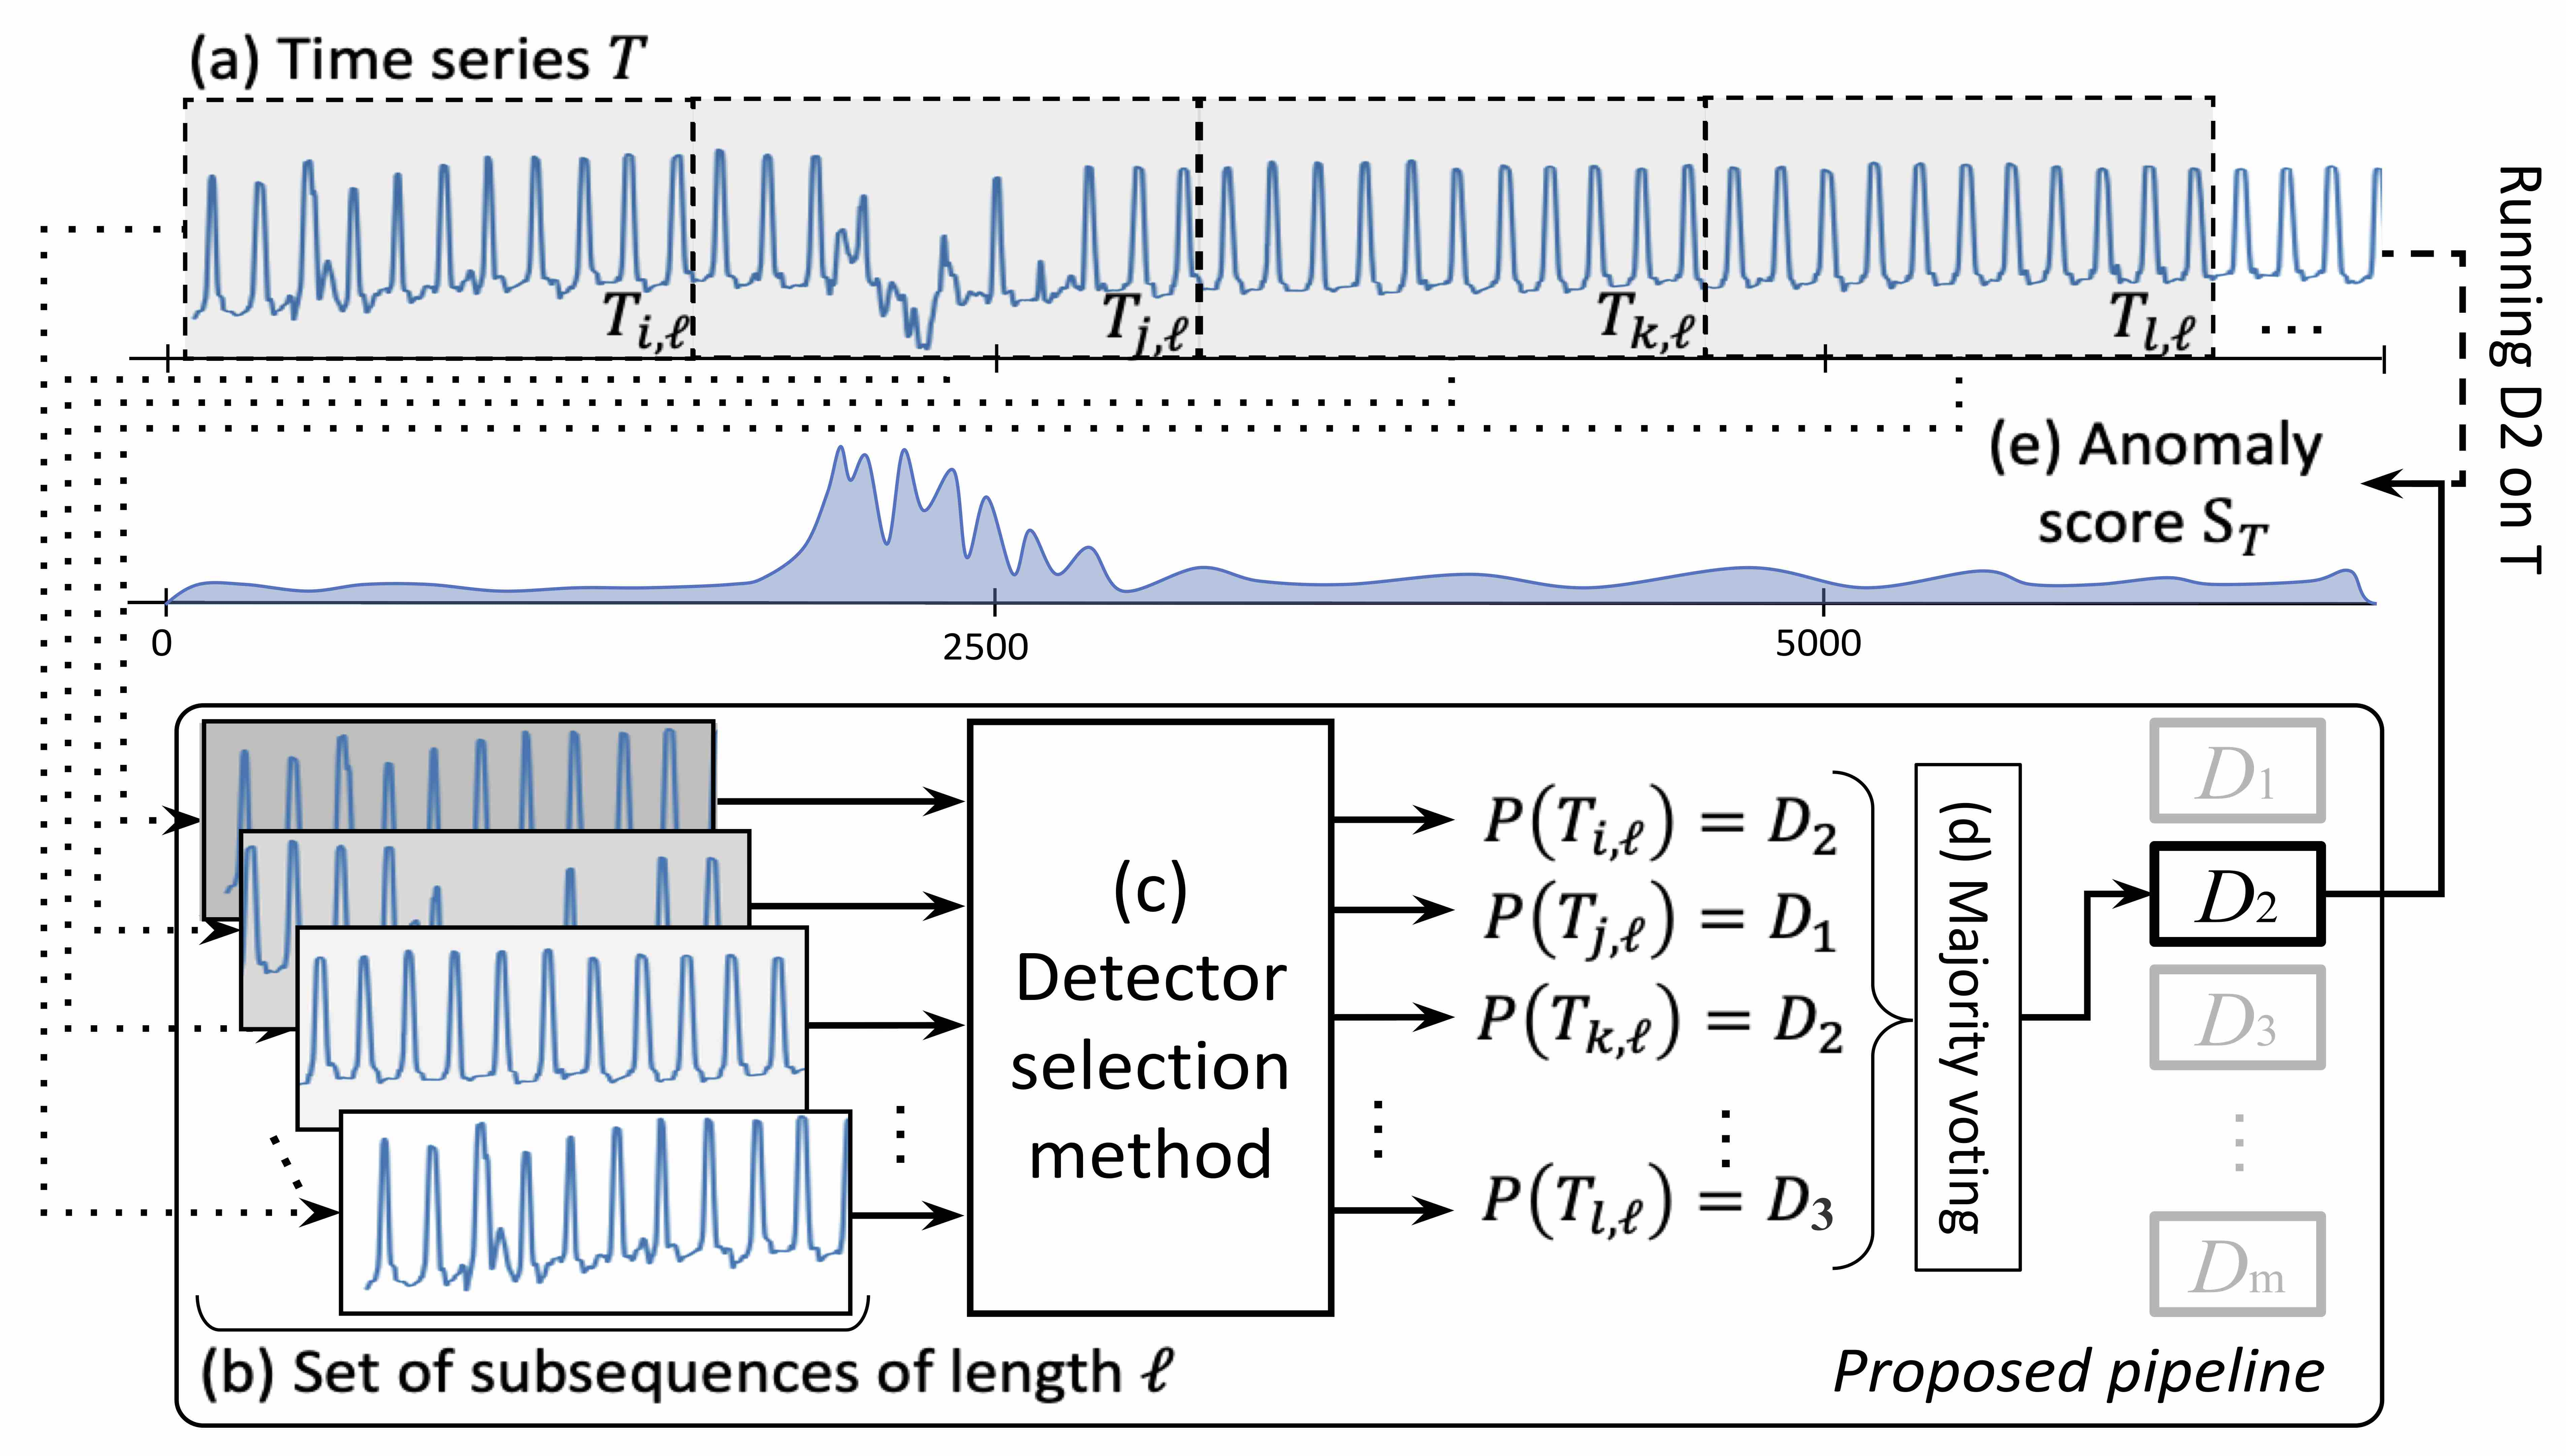
\includegraphics[width=1\linewidth]{figures/Fig3.jpg}
    \caption{Proposed pipeline for the method selection}
    \label{fig:proposed_work}
\end{figure}

In the following section, we provide a comprehensive explanation of the proposed pipeline. This pipeline corresponds to a sequence of preprocessing and postprocessing steps such that the inputs of the model selection algorithms are equal in length. The proposed pipeline, illustrated in Figure~\ref{fig:proposed_work}, is composed of the following steps: (i) \textbf{Preprocessing step}: Extraction of the subsequences of same lengths (Figure~\ref{fig:proposed_work} (b)), (ii) \textbf{Prediction step}: Prediction of which detector to use for each subsequence (Figure~\ref{fig:proposed_work} (c)), and (iii) \textbf{Selection step}: Majority voting among all the different prediction to select one detector only (Figure~\ref{fig:proposed_work} (d)). In the following section, we describe the three steps mentioned above in detail.

\subsection{Preprocessing Step}
Time series classification can be performed with three different strategies: (i) treating the entire time series as one sample, (ii) dividing the time series into overlapping subsequences, (iii) dividing the time series into shifting subsequences (i.e., non-overlapping subsequences). The first strategy is straightforward, as each time series is treated as a single observation. Nevertheless, not all classifiers can handle variable-length inputs, and training such models can be computationally intensive (i.e., batches of time series cannot be treated in parallel). The second strategy involves dividing the time series into overlapping subsequences (of a given window length $\ell$). Despite possible loss of information, it forces each input of the methods to be the same length ($\ell$), allowing simpler and faster computation when performed in parallel. In the third strategy, we divide time series into non-overlapping subsequences (of a given length $\ell$), removing redundant information in overlapping subsequences. The latter might lead to separate anomalies into multiple windows, but significantly reduces the number of inputs generated by the second strategy and significantly accelerates the training and inference time. For these reasons, we chose the third strategy.

Thus, the time series of length $|T|$ are divided into $\mathbb{T}_l$ non-overlapping subsequences of length $\ell$. When the length of the time series is not divided evenly with the window length $\ell$, the remainder is added with an overlap between the first two windows. Formally, $\mathbb{T}_l$ is defined as follows:
\journalv{\begin{equation*}
    \mathbb{T}_\ell = 
    \begin{cases}
        \begin{aligned}
            &\big\{ T_{i*\ell,\ell} \,\big|\, \forall i \in \big[0,\big\lceil \frac{|T|}{\ell} \big\rceil \big] \big\} \\
            &\quad \text{, if } \big\lceil \frac{|T|}{\ell} \big\rceil = \frac{|T|}{\ell}
        \end{aligned} \\
        \begin{aligned}
            &\big\{ T_{0,\ell} \big\} \cup \big\{ T_{|T| - \lceil \frac{|T|}{\ell} \rceil + i*\ell,\ell} \,\big|\, \forall i \in \big[0,\big\lceil \frac{|T|}{\ell} \big\rceil \big] \big\} \\
            &\quad \text{, if } \big\lceil \frac{|T|}{\ell} \big\rceil < \frac{|T|}{\ell}
        \end{aligned}
    \end{cases}
\end{equation*}}
We expect the length $\ell$ to have an impact on the anomaly detection accuracy. We thus test multiple length values and measure their influence (on accuracy and execution time) in Section~\ref{sec:exp}.

At this point, we preprocessed the time series into subsequences of equal length. We now discuss the label (i.e., the best detector to apply) attribution. For that matter, we use the TSB-UAD benchmark~\cite{10.14778/3529337.3529354} that contains 12 different anomaly detection methods. We compute the 12 methods for each time series and attribute the most accurate (based on AUC-PR) detector as the label. Then, the produced subsequences share the same label as the time series they originate from. This labeled dataset can be used to train classification methods and divided into the train, test, and validation sets. It is important to note that although each time series produces multiple samples (i.e., subsequences), these samples should not be mixed between train, validation, and test set. Indeed, too strong similarities between subsequences that belong to the same time series, if contained in both the train, validation and the test, can lead the classification model to overfit or create an illusion of accuracy. Therefore, we guarantee that the intersection between the train, validation, and test set, regarding which time series the corresponding subsequences originate from, is empty.

\subsection{Time Series Classification Approaches}

In this section, we describe the time series classifier approaches that we use as model selection methods. As many approaches have been proposed in the literature, we restrict our experimental evaluation to two main categories: (i) feature-based and (ii) raw-based methods. In addition, the second category can be divided into two sub-categories: (i) convolutional-based and (ii) transformer-based. \journalv{It is worth noting that raw-based methods also utilize features for classification, although the extraction of these features is performed automatically within the network. Despite this, we classify them as raw-based due to the nature of their input.} Figure~\ref{fig:taxonomy} illustrates a simplified taxonomy of the methods considered, and we describe them in the following section.

\subsubsection{Feature-based classification}
The main idea regarding feature-based classification is to use the dataset of time series (or subsequences of time series) to create a dataset whose samples are described by features common to all samples. Using the feature-based dataset, we then employ traditional machine learning classifiers to classify each time series. We use the TSFresh~\cite{CHRIST201872} (Time Series Feature extraction based on scalable hypothesis tests) to extract each subsequence's features. The latter is used for automated time series feature extraction and selection based on the FRESH algorithm~\cite{christ2016distributed}. More specifically, it automatically selects relevant features for a specific task. This is achieved using statistical tests, time series heuristics, and machine learning algorithms. The TSFresh package provides three options for automated feature extraction, namely, (i) \textit{ comprehensive}, (ii) \textit{ efficient}, and (iii) \textit{ minimal}. The first two options provide 700 hundred features and the latter provides only 9. For scalability reasons (the dataset transformation can reach millions of subsequences), we consider the \textit{minimal} option in this paper.

Moreover, the objective is not to evaluate Feature-based classifiers \textit{per se}, but rather to evaluate the ability of TSFresh to extract meaningful features for time series classification (and model selection for anomaly detection, in particular). In this paper, we consider the following classification approaches.

\noindent\textbf{[SVC]}
A Support Vector Classifier (SVC)~\cite{10.1145/130385.130401} is a classifier that maps instances in space in order to maximize the width of the gap between the classes. New instances are mapped into the same space and classified according to which side of the gap they fall. 

\noindent\textbf{[Bayes]}
The naive Bayes classifier~\cite{Zhang2004TheOO} uses Bayes' theorem to predict the class of a new instance based on prior probabilities and class-conditional probabilities. The prediction is made by computing the posterior probabilities for each class.

\noindent\textbf{[MLP]}
A Multi Layer Perceptron (MLP)~\cite{Hinton1989ConnectionistLP} is a fully connected (connections between every neuron) neural network.

\noindent\textbf{[QDA]}
A Quadratic Discriminant Analysis (QDA)~\cite{Geisser1964PosteriorOF} Classifier is a linear discriminant analysis algorithm. The prediction is made by computing the discriminant functions for each class.

\noindent\textbf{[AdaBoost]}
AdaBoost~\cite{10.5555/646943.712093} is a boosting ensemble machine learning algorithm for solving classification problems. It creates a sequence of weak classifiers, where each classifier is trained on a weighted sample of the dataset. The prediction is made by combining the predictions of all classifiers, weighted by their accuracy.

\noindent\textbf{[Decision Tree]}
A Decision Tree Classifier~\cite{Hunt1966ExperimentsII} is a tree-based method that represents a sequence of decisions based on the features of the dataset. To classify a new instance, the algorithm follows the decisions in the tree to reach a leaf node associated with a class.

\noindent\textbf{[Random Forest]}
A Random Forest Classifier~\cite{598994} is an ensemble machine learning algorithm that combines multiple decision trees, where each tree is built using a random subset of the features and a random sample of the data. The final class prediction for a new instance results from the aggregation of the predictions of all trees.

\noindent\textbf{[kNN]}
A kNN classifier~\cite{Fix1989DiscriminatoryA} is a method that classifies instances based on their distance to other instances in a training set. The algorithm assigns the new instances to the class with the most number of closest neighbors among the $K$ nearest data points. 

\subsubsection{Raw-based classification}

Instead of using features to perform classification, the raw values of the time series can be used. Indeed, whereas features are efficient for homogenizing time series datasets (e.g., setting a constant number of features for variable length time series), it might hide important information in the shape of consecutive values. Thus, many approaches that use raw-values time series have been proposed.

\noindent\textbf{[Rocket]}
Among the recent raw-values methods, \journalv{Mini\-Rocket}~\cite{dempster2021minirocket} is one of the state-of-the-art time series classification methods. The latter consists of a feature extraction step and a classification step. More specifically, MiniRocket works by transforming input time series using a small, fixed set of convolutional kernels and using the transformed features to train a logistic regression classifier (using stochastic gradient descent). We refer to MiniRocket as Rocket.

\subsubsection{Convolutional-based classification}

Convolutional-based approaches take as input raw-values of time series and have been shown to be accurate for time series classification~\cite{DBLP:conf/sigmod/BoniolMRP22}.

\noindent\textbf{[ConvNet]}
A Convolutional Neural Network (CNN) \cite{DBLP:journals/corr/OSheaN15} is a type of deep learning neural network widely used in image recognition that is specially designed to extract patterns through data with a grid-like structure, such as images, or time series. A CNN uses convolution, where a filter is applied to a sliding window over the time series. The ConvNet architecture proposed in~\cite{DBLP:journals/corr/WangYO16} is composed of three stacked Convolutional blocks followed by Global Average Pooling (GAP), and a Softmax activation function. Each Convolutional block is composed of a convolutional layer (used with a kernel length of $3$) followed by a batch normalization layer, followed by a ReLU activation function is applied.

\noindent\textbf{[ResNet]}
The Residual Network (ResNet) architecture~\cite{https://doi.org/10.48550/arxiv.1512.03385} was introduced to address the gradient vanishing problem encountered in large CNNs~\cite{simonyan2015a}. A ResNet is composed of several blocks connected together with residual connections (i.e., identity mapping). For time series classification, a ResNet architecture has been proposed in~\cite{DBLP:journals/corr/WangYO16}, and has demonstrated strong classification accuracy~\cite{fawaz2019deep}. It is the same architecture as the previously described ConvNet, with additional residual connections between convolutional blocks.

\noindent\textbf{[InceptionTime]}
The model consists of a network using residual connections and convolutional layers with kernels of variable lengths~\cite{fawaz2020inceptiontime}. Such a network uses three Inception blocks that replace the traditional residual blocks that we can find in a ResNet architecture. Each Inception block consists of a concatenation of convolutional layers using different sizes of filters. For each block, the time series is fed to three different 1D convolutional layers with different kernel sizes (10, 20, and 40) and one Max-Pooling layer with kernel size 3. The last step consists of concatenating the previous four layers along the channel dimension and applying a ReLU activation function to the output, followed by batch normalization. The convolutional layers have 32 filters and a stride parameter of 1.

\subsubsection{Transformer-based classification}

%The second category, initially introduced for computer vision tasks~\cite{vaswani2017attention,dosovitskiy2020image}, is Transformer-based approaches. 
Transformer-based approaches were initially introduced for Natural Language Processing~\cite{vaswani2017attention}. Such methods can easily be adapted for time series classification tasks, and in this paper we propose SiT (Signal Transformer), an extension of a recent computer vision transformer approach~\cite{dosovitskiy2020image}. SiT first starts by projecting the input to the latent space with an embedding step. After the embedding step, the input is mapped to a $D$ dimensional space (we use $D=256$ in the rest of the paper) that serves as input to an encoder. For SiT, we use an encoder originally proposed for computer vision tasks~\cite{vaswani2017attention} that consists of multiple blocks. Each block has an alternating multi-headed self-attention block and a feed-forward layer, both preceded by a normalization step and a residual connection. We now describe the different embedding steps in detail in the following paragraphs. In the experimental evaluation, we consider the SiT architecture with the four embeddings as four different methods.

\noindent\textbf{[SiT-conv]}
This embedding uses a single convolutional layer to map the time series into the latent space. The convolutional layer has a kernel and stride of the same length (we use a length of 16 throughout the rest of the paper), essentially taking non-overlapping steps over the time series. Finally, the convolutional layer has $D$ filters to match the input dimension of the SiT encoder.

\noindent\textbf{[SiT-linear]}
The linear embedding~\cite{dosovitskiy2020image} splits the input time-series into non-overlapping subsequences of length $l_{SiT}$ (we use $l_{SiT}=16$ in the rest of the paper). Then, each patch is linearly projected into $D$ dimensions to match the input dimension of the SiT encoder.

\noindent\textbf{[SiT-stem]}
The stem embedding~\cite{xiao2021early} consists of 3 convolutional layers with a kernel length of 3, a stride length of 2, and a number of filters equal to 3, 5, and 7, respectively. These three convolutional layers are then followed by a last convolutional layer with $D$ dimensions and a kernel and stride length equal to 1. This embedding was initially proposed to overcome unstable behavior while training because of its early visual processing step. 

\noindent\textbf{[SiT-stem-ReLU]}
Similarly to the previous embedding, the stem-ReLU embedding~\cite{wang2022scaled} consists of 4 convolutional layers with kernel lengths of 7, 3, 3, 8, stride lengths of 2, 1, 1, 8, and padding of 3, 1, 1, 0. The number of filters for each convolutional layer is 3, except the last one with $D$ filters to match the SiT encoder's dimension.

\begin{figure}
    \centering
    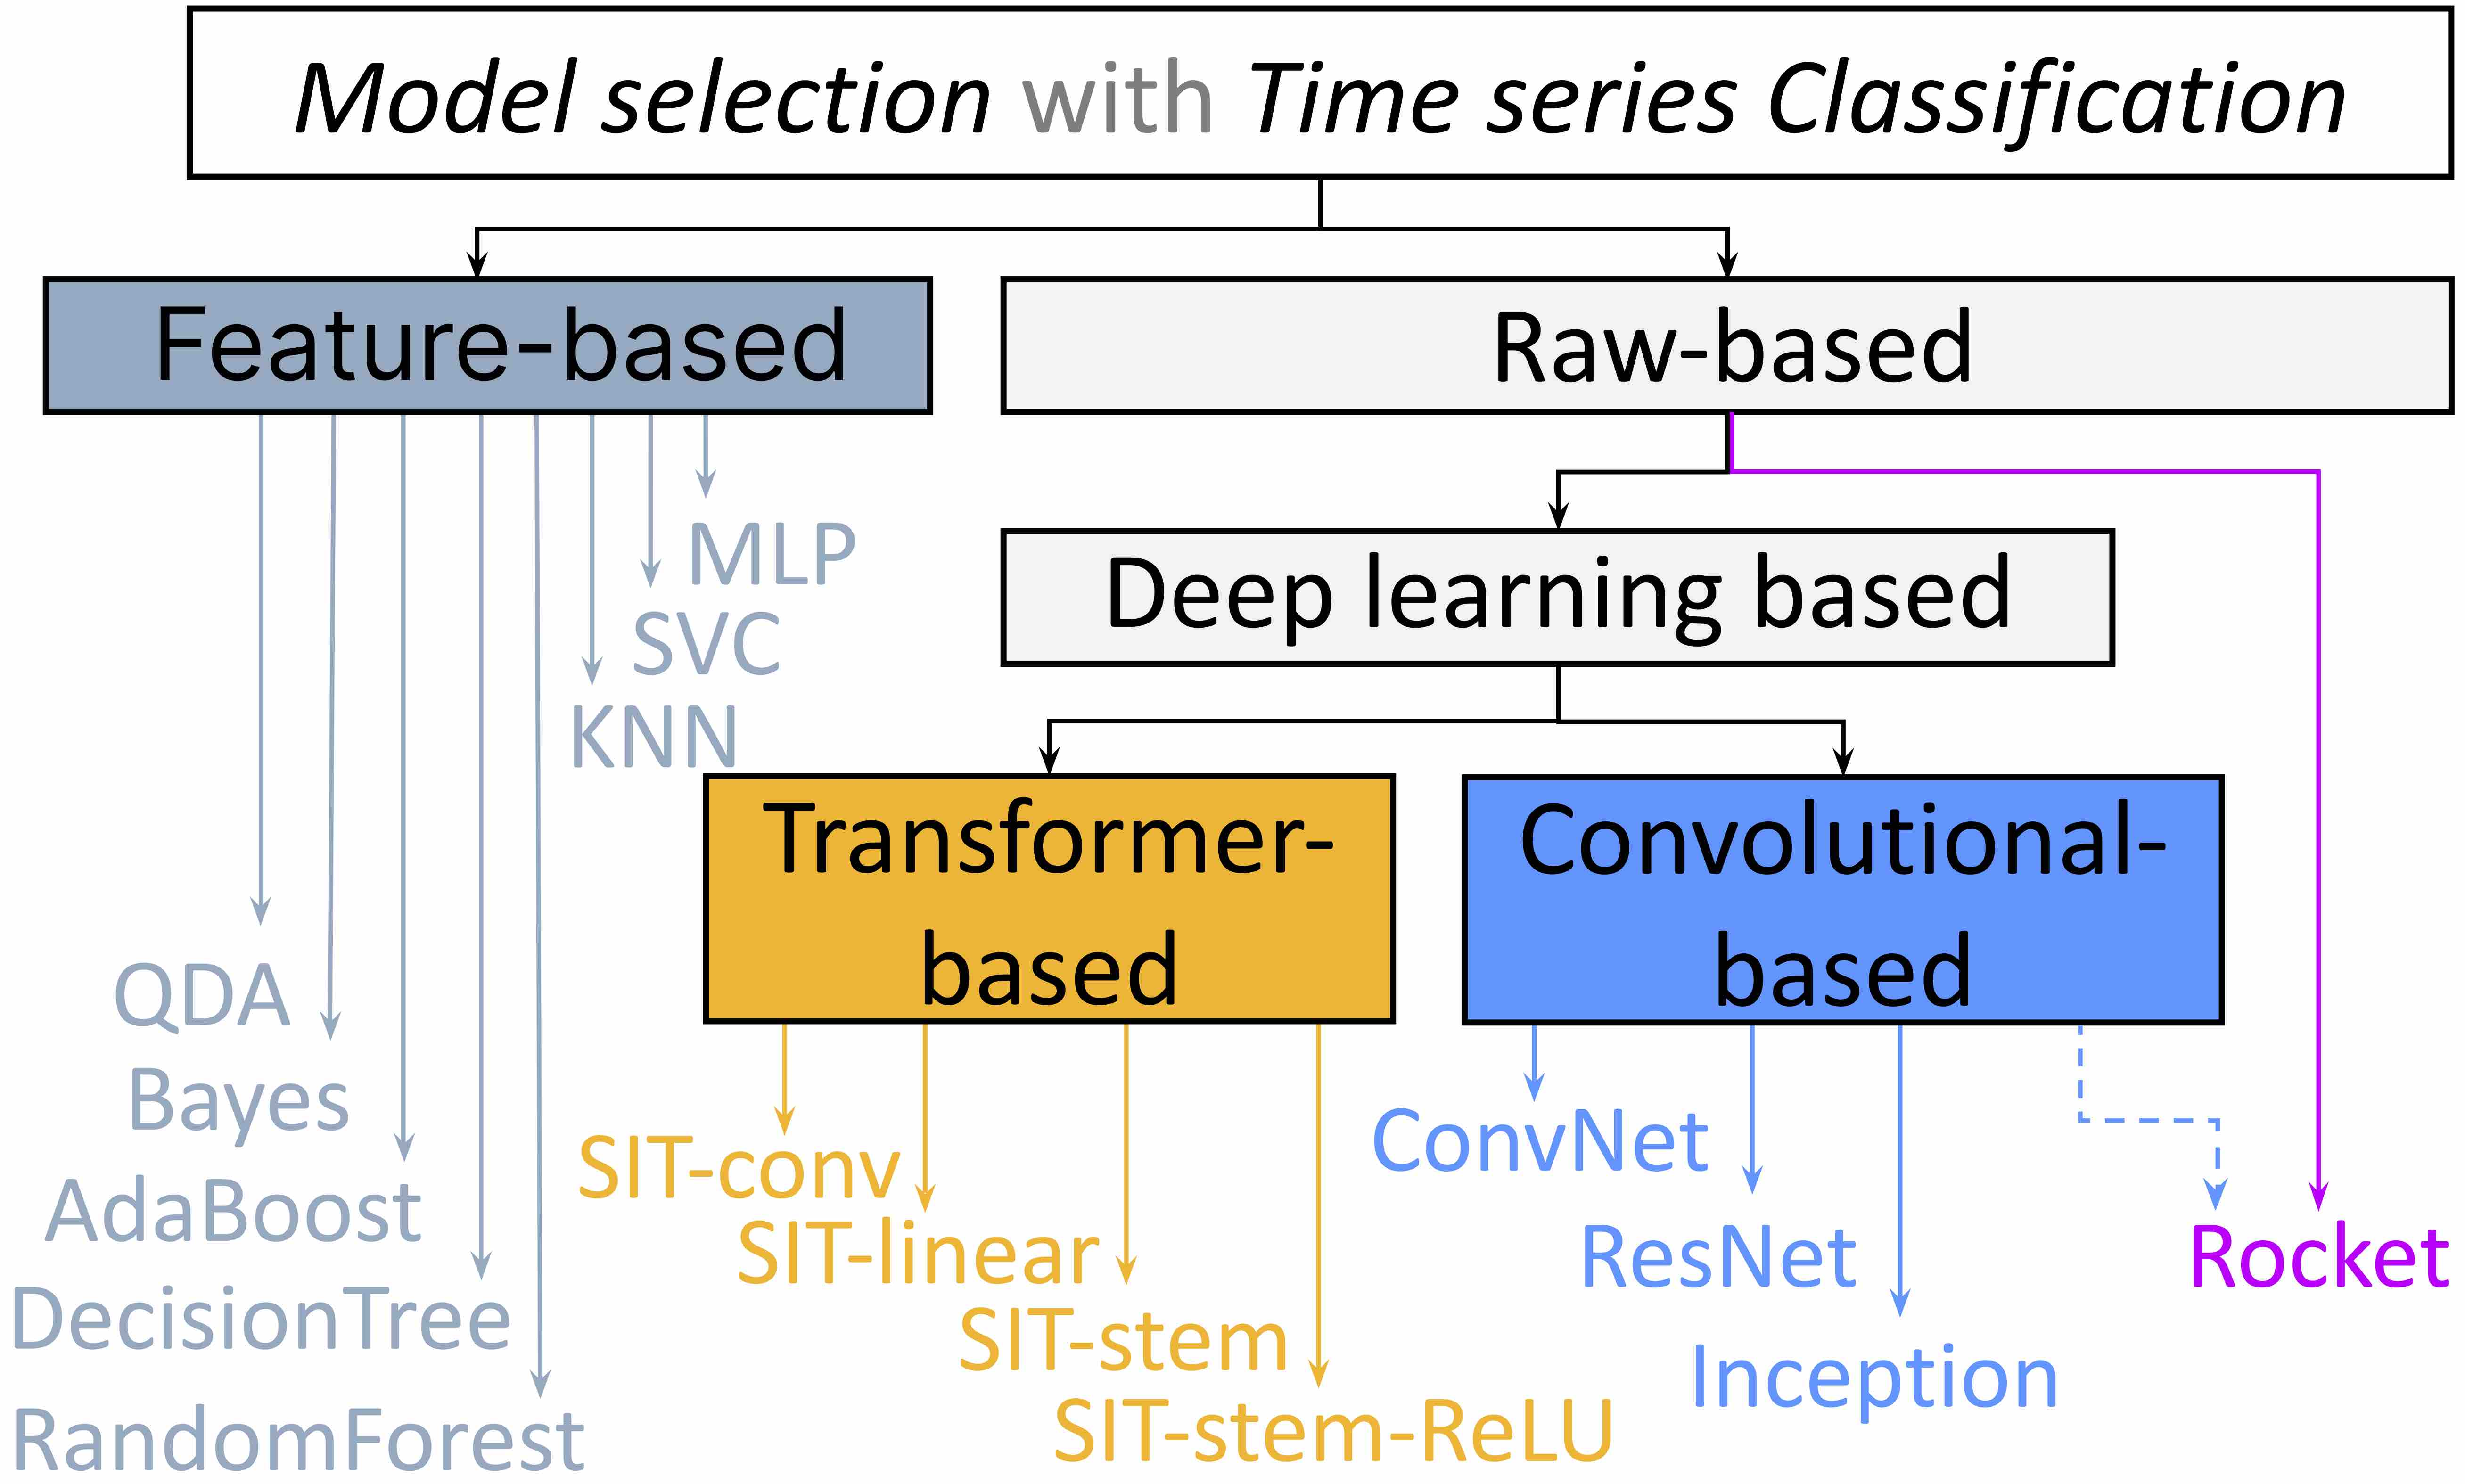
\includegraphics[width=1\linewidth]{figures/Fig4.jpg}
    \caption{Taxonomy of time series classification approaches used as model selection methods. We use the same color code for each class in all figures in the paper.}
    \label{fig:taxonomy}
\end{figure}


\subsection{Selecting the Detector}

We train the time series classification methods mentioned in the previous section to predict the best detector for each subsequence (as shown in Figure~\ref{fig:proposed_work} (c)). However, there is no guarantee that the classification model selects the same detector for all subsequences. Therefore, we choose the best detector for one time series by doing a majority voting step between the predictions for every subsequence, such that the most voted detector is selected as the detector of the time series. Formally, given a classification model $\mathcal{M}_{cl}$ applied on a given time series $T$ subsequences $\mathbb{T}_\ell$, we define $\mathcal{M}_{cl}(\mathbb{T}_\ell)$ the set of model selected for each subsequence in $\mathbb{T}_\ell$. Therefore, we define the majority voting function as follows:
\begin{equation*}
     f_{MV}(T,\mathcal{M}_{cl}) = \operatorname*{argmax}_{D \in \mathcal{M}_{cl}(\mathbb{T}_\ell)} \sum_{T_{i, \ell} \in \mathbb{T}_\ell} \mathds{1}_{[\mathcal{M}_{cl}(T_{i, \ell}) = D]}
\end{equation*}

Majority voting serves the pipeline with two significant factors, (i) it does not depend on the design of the detector and makes the pipeline easily usable for multiple different types of anomaly detection methods, and (ii) majority voting averages the predictions and reduces the impact of misclassified subsequences. To conclude, in our pipeline, the model selection method introduced in Problem~\ref{prob:probdef} is the output of $f_{MV}(T,\mathcal{M}_{cl})$.
\section{Experimental Evaluation}
\label{sec:exp}

We now describe in detail our experimental analysis. For additional information, we make all our material publicly available online~\cite{ourcode} and provide an interactive WebApp~\cite{ourwebsite} for navigating and exploring the experimental results.

\journalv{The experimental section is organized as follows:
\begin{itemize}%[noitemsep,topsep=0pt,parsep=0pt,partopsep=0pt,leftmargin=0.5cm]
    \item In \textbf{Section~\ref{exp:setup}}, we first start by introducing the datasets and the methods to evaluate the previously defined model selection baselines. We also define the performance measures.
    \item In \textbf{Section~\ref{exp:overalleval}}, we then conduct an extensive evaluation of both accuracy (classification and anomaly detection) and execution time for all model selection methods and over the entire benchmark.
    \item In \textbf{Section~\ref{exp:windowlength}}, we analyze more precisely the influence of the window length of our proposed pipeline.
    \item In \textbf{Section~\ref{exp:datasets}}, we measure the influence of datasets and anomalies characteristics on the performances of the model selection algorithms.
    \item In \textbf{Section~\ref{exp:detectionvsclass}}, we measure the correlation between classification accuracy (i.e., of the model selection methods) and anomaly detection accuracy. We proposed empirical lower and upper bounds that contain the minimal and the maximal performances of any model selection algorithms for a given classification accuracy.
    \item In \textbf{Section~\ref{exp:sup2unsup}}, we finally measure the accuracy of model selection methods when used in an unsupervised manner (i.e., used for time series from domains that were not included in the training set). 
\end{itemize}}

\journalv{\subsection{Experimental Setup and Settings}}
\label{exp:setup}

\begin{table*}[tb]
    \centering
    \caption{\journalv{Summary of datasets, methods, and measures used in this experimental evaluation.}}
        \scalebox{0.8}{
        \begin{tabular}{|c|c|}
        \hline
        \rowcolor{Gray}
        \textbf{Datasets} & \textbf{Description} \\
        \hline
        Dodgers~\cite{10.1145/1150402.1150428} & unusual traffic after a Dodgers game \textbf{(1 time series)}\\ 
        \hline
        ECG~\cite{Moody} & standard electrocardiogram dataset \textbf{(52 time series)}\\ 
        \hline
        IOPS~\cite{IOPS} & performance indicators of a machine \textbf{(58 time series)}\\ 
        \hline
        KDD21~\cite{kdd21} & composite dataset released in a recent SIGKDD 2021 \textbf{(250 time series)}\\ 
        \hline
        MGAB~\cite{markus_thill_2020_3762385} & Mackey-Glass time series with non-trivial anomalies \textbf{(10 time series)}\\ 
        \hline
        NAB~\cite{ahmad_unsupervised_2017} &  Web-related real-world and artificial time series \textbf{(58 time series)}\\ 
        \hline
        SensorScope~\cite{YAO20101059} & environmental data \textbf{(23 time series)}\\ 
        \hline
        YAHOO~\cite{yahoo} & \makecell{ time series based on Yahoo production systems \textbf{(367 time series)}}\\ 
        \hline
        Daphnet~\cite{5325884} & acceleration sensors on Parkinson's disease patients \textbf{(45 time series)}\\ 
        \hline
        GHL~\cite{filonov2016multivariate} & Gasoil Heating Loop telemetry \textbf{(126 time series)}\\ 
        \hline
        Genesis~\cite{vonBirgelen2018} & portable pick-and-place demonstrator \textbf{(6 time series)}\\ 
        \hline
        MITDB~\cite{Moody} & ambulatory ECG recordings \textbf{(32 time series)}\\ 
        \hline
        OPPORTUNITY~\cite{5573462} & motion sensors for human activity recognition \textbf{(465 time series)}\\ 
        \hline
        Occupancy~\cite{CANDANEDO201628} & temperature, humidity, light, and CO2 of a room \textbf{(10 time series)}\\ 
        \hline
        SMD~\cite{10.1145/3292500.3330672} & Server Machine telemetry \textbf{(281 time series)}\\ 
        \hline
        SVDB~\cite{greenwald_improved_1990} & ECG recordings \textbf{(115 time series)}\\ 
        \hline
        \hline
        \rowcolor{Gray}
        \textbf{Anomaly Detection} & \textbf{Description} \\
        \hline
        IForest~\cite{liu_isolation_2008} & \makecell{constructs binary trees based on random space splitting. The nodes (i.e., \\ subsequences) with shorter paths to the root are more likely to be anomalies. }\\
        \hline
        IForest1~\cite{liu_isolation_2008}  & same as IForest, but each point (individually) are used as input. \\
        \hline
        LOF~\cite{Breunig:2000:LID:342009.335388} & computes the ratio of the neighboring density to the local density.\\ 
        \hline
        MP~\cite{yeh_time_2018} & \makecell{detects abnormal subsequences with the largest nearest neighbor distance.} \\ 
        \hline
        NormA~\cite{boniol_unsupervised_2021} & \makecell{identifies normal patterns using clustering and calculates each subsequence \\ weighted distance (with statistical criteria) to the normal patterns.} \\ 
        \hline
        PCA~\cite{aggarwal_outlier_2017} & \makecell{projects data to a lower-dimensional hyperplane, and data points \\ with a significant distance from this plane can be identified as outliers.} \\ 
        \hline
        AE~\cite{10.1145/2689746.2689747} & \makecell{projects data to the lower-dimensional latent space and reconstructs the \\ data, and outliers are expected to have larger reconstruction errors.} \\ 
        \hline
        LSTM-AD~\cite{malhotra_long_2015} & \makecell{use an LSTM network that from the current subsequence tries to predict the \\ following value. The error prediction is then used to identify anomalies.}\\ 
        \hline
        POLY~\cite{li_unifying_2007} & \makecell{fits a polynomial model that tries to predict the time series values from the \\ previous subsequences. Outliers are detected with prediction error} \\ 
        \hline
        CNN~\cite{8581424} & \makecell{builds, using a convolutional neural network, a correlation between current \\ and previous subsequences. The anomaly score is the prediction deviation.} \\ 
        \hline
        OCSVM~\cite{scholkopf_support_1999} & \makecell{is a support vector method that fits the normal training dataset and finds the normal data's boundary.}\\ 
        \hline
        HBOS~\cite{goldstein2012histogram} & \makecell{builds a histogram for the time series. The anomaly score is the  inverse of the height of the bin.} \\
        \hline
        \hline
        \rowcolor{Gray}
        \textbf{Model Selection} & \textbf{Description} \\
        \hline
            % \rowcolor{lGray}
            % \multicolumn{2}{|c|}{\it Feature-based classifier} \\
            % \hline \trianbox1{featurebased}
        \cellcolor{featurebased} SVC~\cite{10.1145/130385.130401} &  \makecell{maps instances to points in space to maximize the gap between classes.}\\
        \hline
        \cellcolor{featurebased} Bayes~\cite{Zhang2004TheOO} & \makecell{uses Bayes' theorem to classify a point using each class posterior probabilities.} \\
        \hline
        \cellcolor{featurebased} MLP~\cite{Hinton1989ConnectionistLP} & \makecell{consists of multiple layers of interconnected neurons} \\
        \hline
        \cellcolor{featurebased} QDA~\cite{Geisser1964PosteriorOF} & is a discriminant analysis algorithm for classification problems \\
        \hline
        \cellcolor{featurebased} AdaBoost~\cite{10.5555/646943.712093} & \makecell{is a meta-algorithm using boosting technique with weak classifiers} \\
        \hline
        \cellcolor{featurebased} Decision Tree~\cite{Hunt1966ExperimentsII} & \makecell{is an approach that splits data points into separate leaves based on features} \\
        \hline
        \cellcolor{featurebased} Random Forest~\cite{598994} & \makecell{is a set of Decision Trees fed with random samples and features.} \\
        \hline
        \cellcolor{featurebased} kNN~\cite{Fix1989DiscriminatoryA} & \makecell{assigns the most common class among its k nearest neighbors.} \\
            % \hline
            % \rowcolor{lGray}
            % \multicolumn{2}{|c|}{\it Time series classifier} \\
        \hline
        \cellcolor{rocket} Rocket~\cite{dempster2021minirocket} & \makecell{transforms time series using a set of convolutional kernels, creating features used to train a linear classifier} \\
        \hline
            % \rowcolor{lGray}
            % \multicolumn{2}{|c|}{\it Convolutional-based neural networks}  \\
            % \hline
        \cellcolor{convbased} ConvNet~\cite{DBLP:journals/corr/WangYO16} & \makecell{uses convolutional layers to learn spatial features from the input data.} \\
        \hline
        \cellcolor{convbased} ResNet~\cite{DBLP:journals/corr/WangYO16} & \makecell{is a ConvNet with residual connections between convolutional block} \\
        \hline
        \cellcolor{convbased} Inception Time~\cite{fawaz2020inceptiontime} & \makecell{is a combination of ResNets with kernels of multiple sizes} \\
        \hline
            % \rowcolor{lGray}
            % \multicolumn{2}{|c|}{\it Transformer-based neural networks}  \\
            % \hline
        \cellcolor{transbased} SiT-conv~\cite{dosovitskiy2020image} & \makecell{is a transformer architecture with a convolutional layer as input} \\
        \hline
        \cellcolor{transbased} SiT-linear~\cite{dosovitskiy2020image} & \makecell{is a transformer architecture for which time series are divided into \\ non-overlapping patches and linearly projected into the embedding space} \\
        \hline
        \cellcolor{transbased} SiT-stem~\cite{xiao2021early} & \makecell{is a transformer architecture with convolutional layers with increasing dimensionality as input} \\
        \hline
        \cellcolor{transbased} SiT-stem-ReLU~\cite{wang2022scaled} & \makecell{is similar to SiT-stem but with Scaled ReLU.} \\
        \hline
        \hline
        \rowcolor{Gray}
        \textbf{\journalv{Evaluation}} & \textbf{\journalv{Description}} \\
        \hline
        Classification Accuracy &  \makecell{the number of correctly selected methods divided by the total number of time series}\\
        \hline
        % \rowcolor{lGray}
        % \multicolumn{2}{|c|}{\it Anomaly detection accuracy measures}  \\
        % \hline
        AUC-PR~\cite{10.1145/1143844.1143874} &  Area under the Precision-Recall curve\\
        \hline
        VUS-PR~\cite{10.14778/3551793.3551830} &  \makecell{Volume under the Precision-Recall surface (obtained from different length of a buffer region surrounding the anomalies)}\\
        \hline
        % \rowcolor{lGray}
        % \multicolumn{2}{|c|}{\it Execution Time measures}  \\
        % \hline
        Training Time & \makecell{number of seconds required to train a model selection method.} \\
        \hline
        Selection Time & \makecell{number of seconds required to predict the best model to use.} \\
        \hline
        Detection Time & \makecell{number of seconds required to compute an anomaly score. For model selection methods, \\it includes both the prediction of the model to use and the execution of the chosen model.} \\
        \hline
        \end{tabular}
        } 
        \label{SymbolTable}
\end{table*}

\noindent \textbf{Technical setup: }
We implemented the deep learning-based model selection methods in Python 3.5 using the PyTorch library~\cite{NEURIPS2019_bdbca288}. For the feature-based approach, we used the TSFresh~\cite{CHRIST201872} and scikit-learn~\cite{JMLR:v12:pedregosa11a} libraries. We then used sktime~\cite{Lning2019sktimeAU} for the Rocket algorithm implementation. For the anomaly detection methods, we used the implementation provided in the TSB-UAD benchmark~\cite{10.14778/3529337.3529354}. The evaluation was conducted on a server with Intel Core i7-8750H CPU 2.20GHz x 12, with 31.3GB RAM, and Quadro P1000/\journalv{PCIe}/SSE2 GPU with 4.2GB RAM, and on Jean Zay cluster with Nvidia Tesla V100 SXM2 GPU with 32 GB RAM.

\noindent \textbf{Datasets: }
For our evaluation purposes, we use the public datasets identified in the TSB-UAD benchmark~\cite{10.14778/3529337.3529354}. The latter corresponds to datasets (described in Table~\ref{SymbolTable}) proposed in the literature containing multiple time series with labeled anomalies. Specifically, each point in every time series is labeled as normal or abnormal.

\noindent \textbf{Anomaly Detection Methods: }
For the experimental evaluation, we select 12 different anomaly detection methods, summarized in Table~\ref{SymbolTable}. Out of these, 8 are fully unsupervised (i.e., they require no prior information on the anomalies to be detected): IForest, IForest1, LOF, MP, NormA, PCA, HBOS, and POLY. The remaining 4 methods are semi-supervised (i.e., they require some information related to normal behaviors), namely, OCSVM, AE, LSTM-AD, and CNN. For all these anomaly detection baselines, we set the parameter as described in the TSB-UAD benchmark~\cite{10.14778/3529337.3529354}.

\noindent \textbf{Method Selection baselines: }
We then consider the method selection baseline described in Section~\ref{sec:proposed} and summarized in Table~\ref{SymbolTable}. We first consider {\it feature-based} methods, that extract features using TSFresh~\cite{CHRIST201872} library to select the correct anomaly detection method. We then consider \journalv{Rocket}, state-of-the-art {\it time series classifier}. We also include two types of deep learning classifiers; (i) {\it Convolutional-based neural networks} and (ii) {\it Transformer-based neural networks}. Table~\ref{SymbolTable} summarizes the different model selection methods (i.e., classifiers). In total, we consider 16 methods, trained with window lengths $\ell$ equal to 16, 32, 64, 128, 256, 512, 768, and 1024. In total, we trained 128 models. In the following section, we refer to a model $M$ trained using a window length $\ell$ as $M$-$\ell$.

\noindent \textbf{Parameter settings: }
We use the same 70/30 split of the benchmark for all the classification models. Therefore, we can compare models trained on the same training set and evaluated on the same set of time series. Then, for the feature-based methods, we set the hyperparameters of the models based on the default parameters of scikit-learn. Moreover, for \journalv{Rocket}, we use 10000 kernels to extract the features and the logistic regression with stochastic gradient descent (computed in batches) for the classification step. Finally, for Convolutional and Transformer-based methods, we use a learning rate of $10^{-5}$, with a batch size of 256 and an early stopping strategy with a maximum of 50 epochs without improvement. Moreover, we use the weighted cross-entropy loss and set the maximum number of epochs to 10,000 (with a training time limit of 20 hours).

\noindent \textbf{Evaluation measures: }
We finally use four evaluation measures\journalv{, summarized in Table~\ref{SymbolTable}}. For model selection accuracy, we use the classification accuracy (i.e., the number of anomaly detectors correctly selected divided by the total number of time series). For anomaly detection accuracy, we use both AUC-PR~\cite{10.1145/1143844.1143874} and VUS-PR~\cite{10.14778/3551793.3551830} (with a buffer length equal to 10 points). For execution time, we measure the {\it training time} (i.e., the time required to train a model selection algorithm), the {\it selection time} (i.e., the time a model selection approach needs to predict which detector to use), and the {\it detection time} (i.e., the time required to predict which detector to use, and to execute it).

\begin{figure}
    \centering
    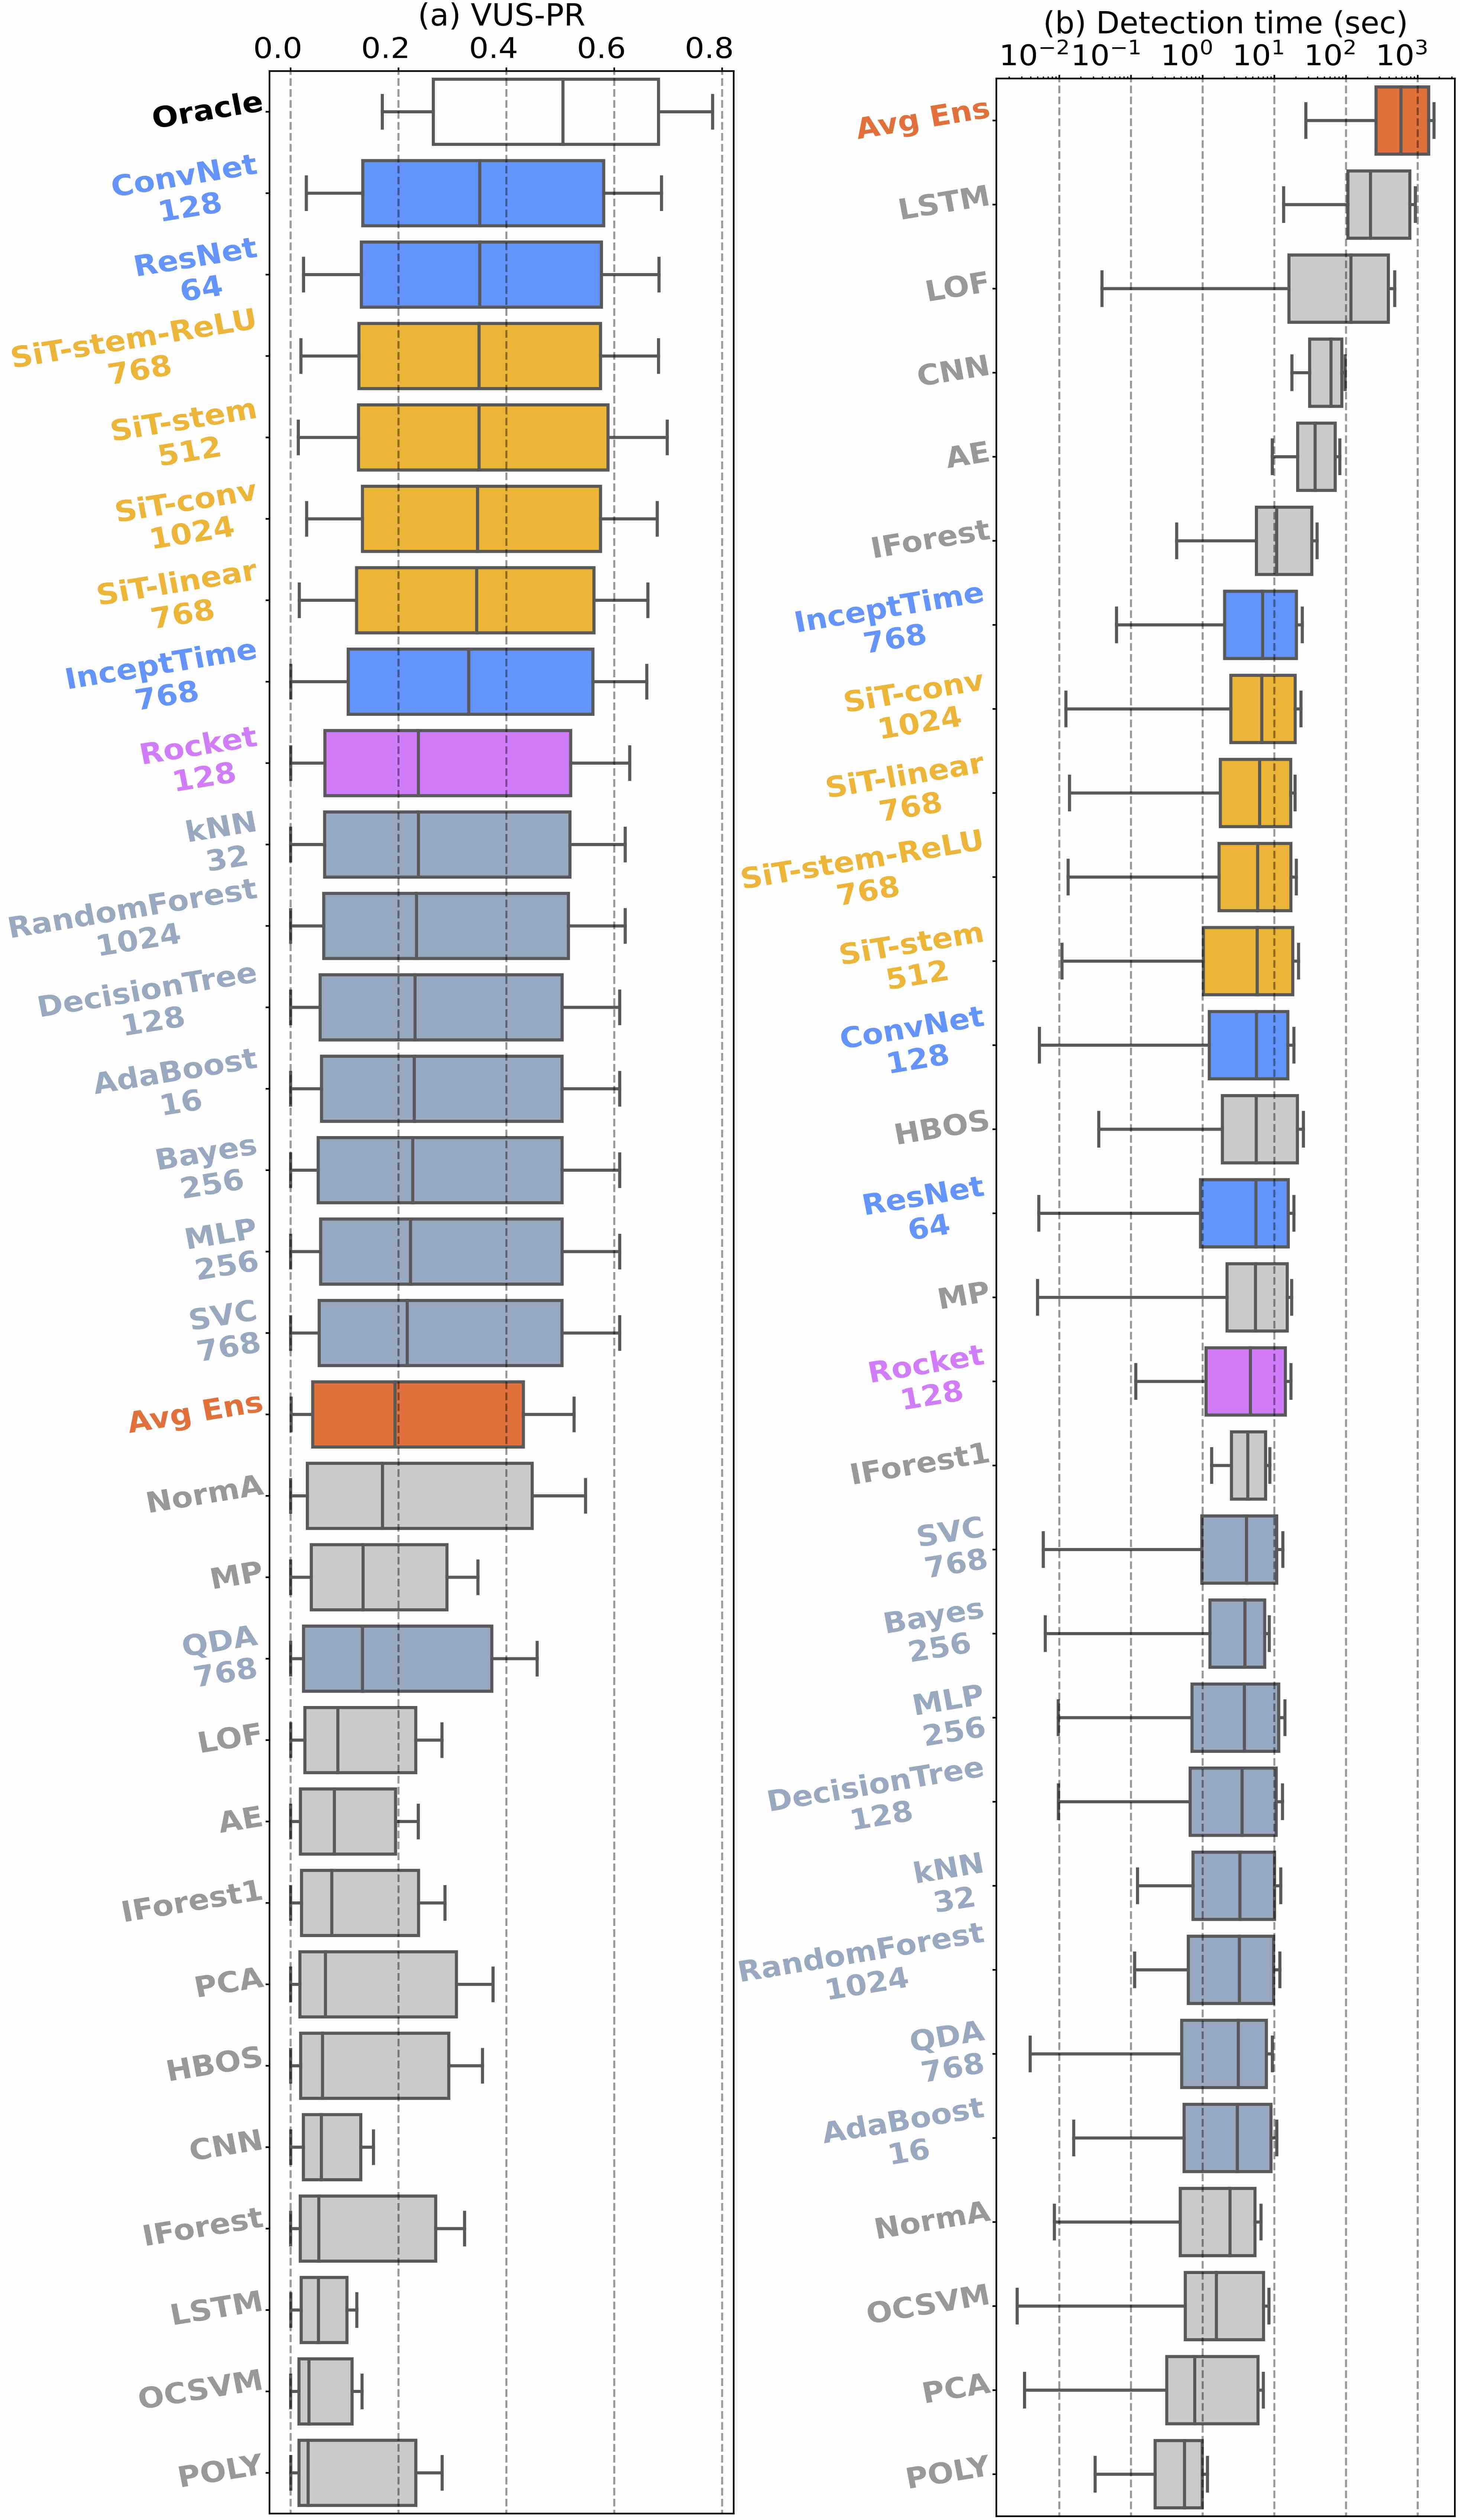
\includegraphics[width=1\linewidth]{figures/Fig5.jpg}
        \caption{VUS-PR and Detection time (seconds) for all model selection approaches (showing only the window length that maximizes VUS-PR for each model) over a test set of 497 series from TSB-UAD. \journalv{The methods are sorted: the most accurate methods are at the top (a); the fastest methods are at the bottom (b)}}
        \label{fig:overall_res}
\end{figure}


\subsection{Overall Evaluation}
\label{exp:overalleval}

We first evaluate accuracy (classification and anomaly detection) and execution time for all model selection methods over the entire benchmark. We split the benchmark into a train and test set with $1404$ and $496$ time series, respectively. Both sets contain time series from all datasets. Thus, the models have examples of all available domains. In Section~\ref{exp:sup2unsup}, we evaluate the performance of the models when applied to unseen (i.e., not used in the training set) datasets.

\subsubsection{\textbf{Accuracy Evaluation}}

We first analyze the accuracy of all model selection methods (using all window lengths) and compare them to the Oracle \journalv{(i.e. the perfect classifier),} the Averaging Ensemble method (Avg Ensemble) \journalv{(i.e., running all anomaly detection methods and returning the average of all anomaly scores),} and \journalv{the} anomaly detection methods in the TSB-UAD benchmark.

\begin{figure}
    \centering
    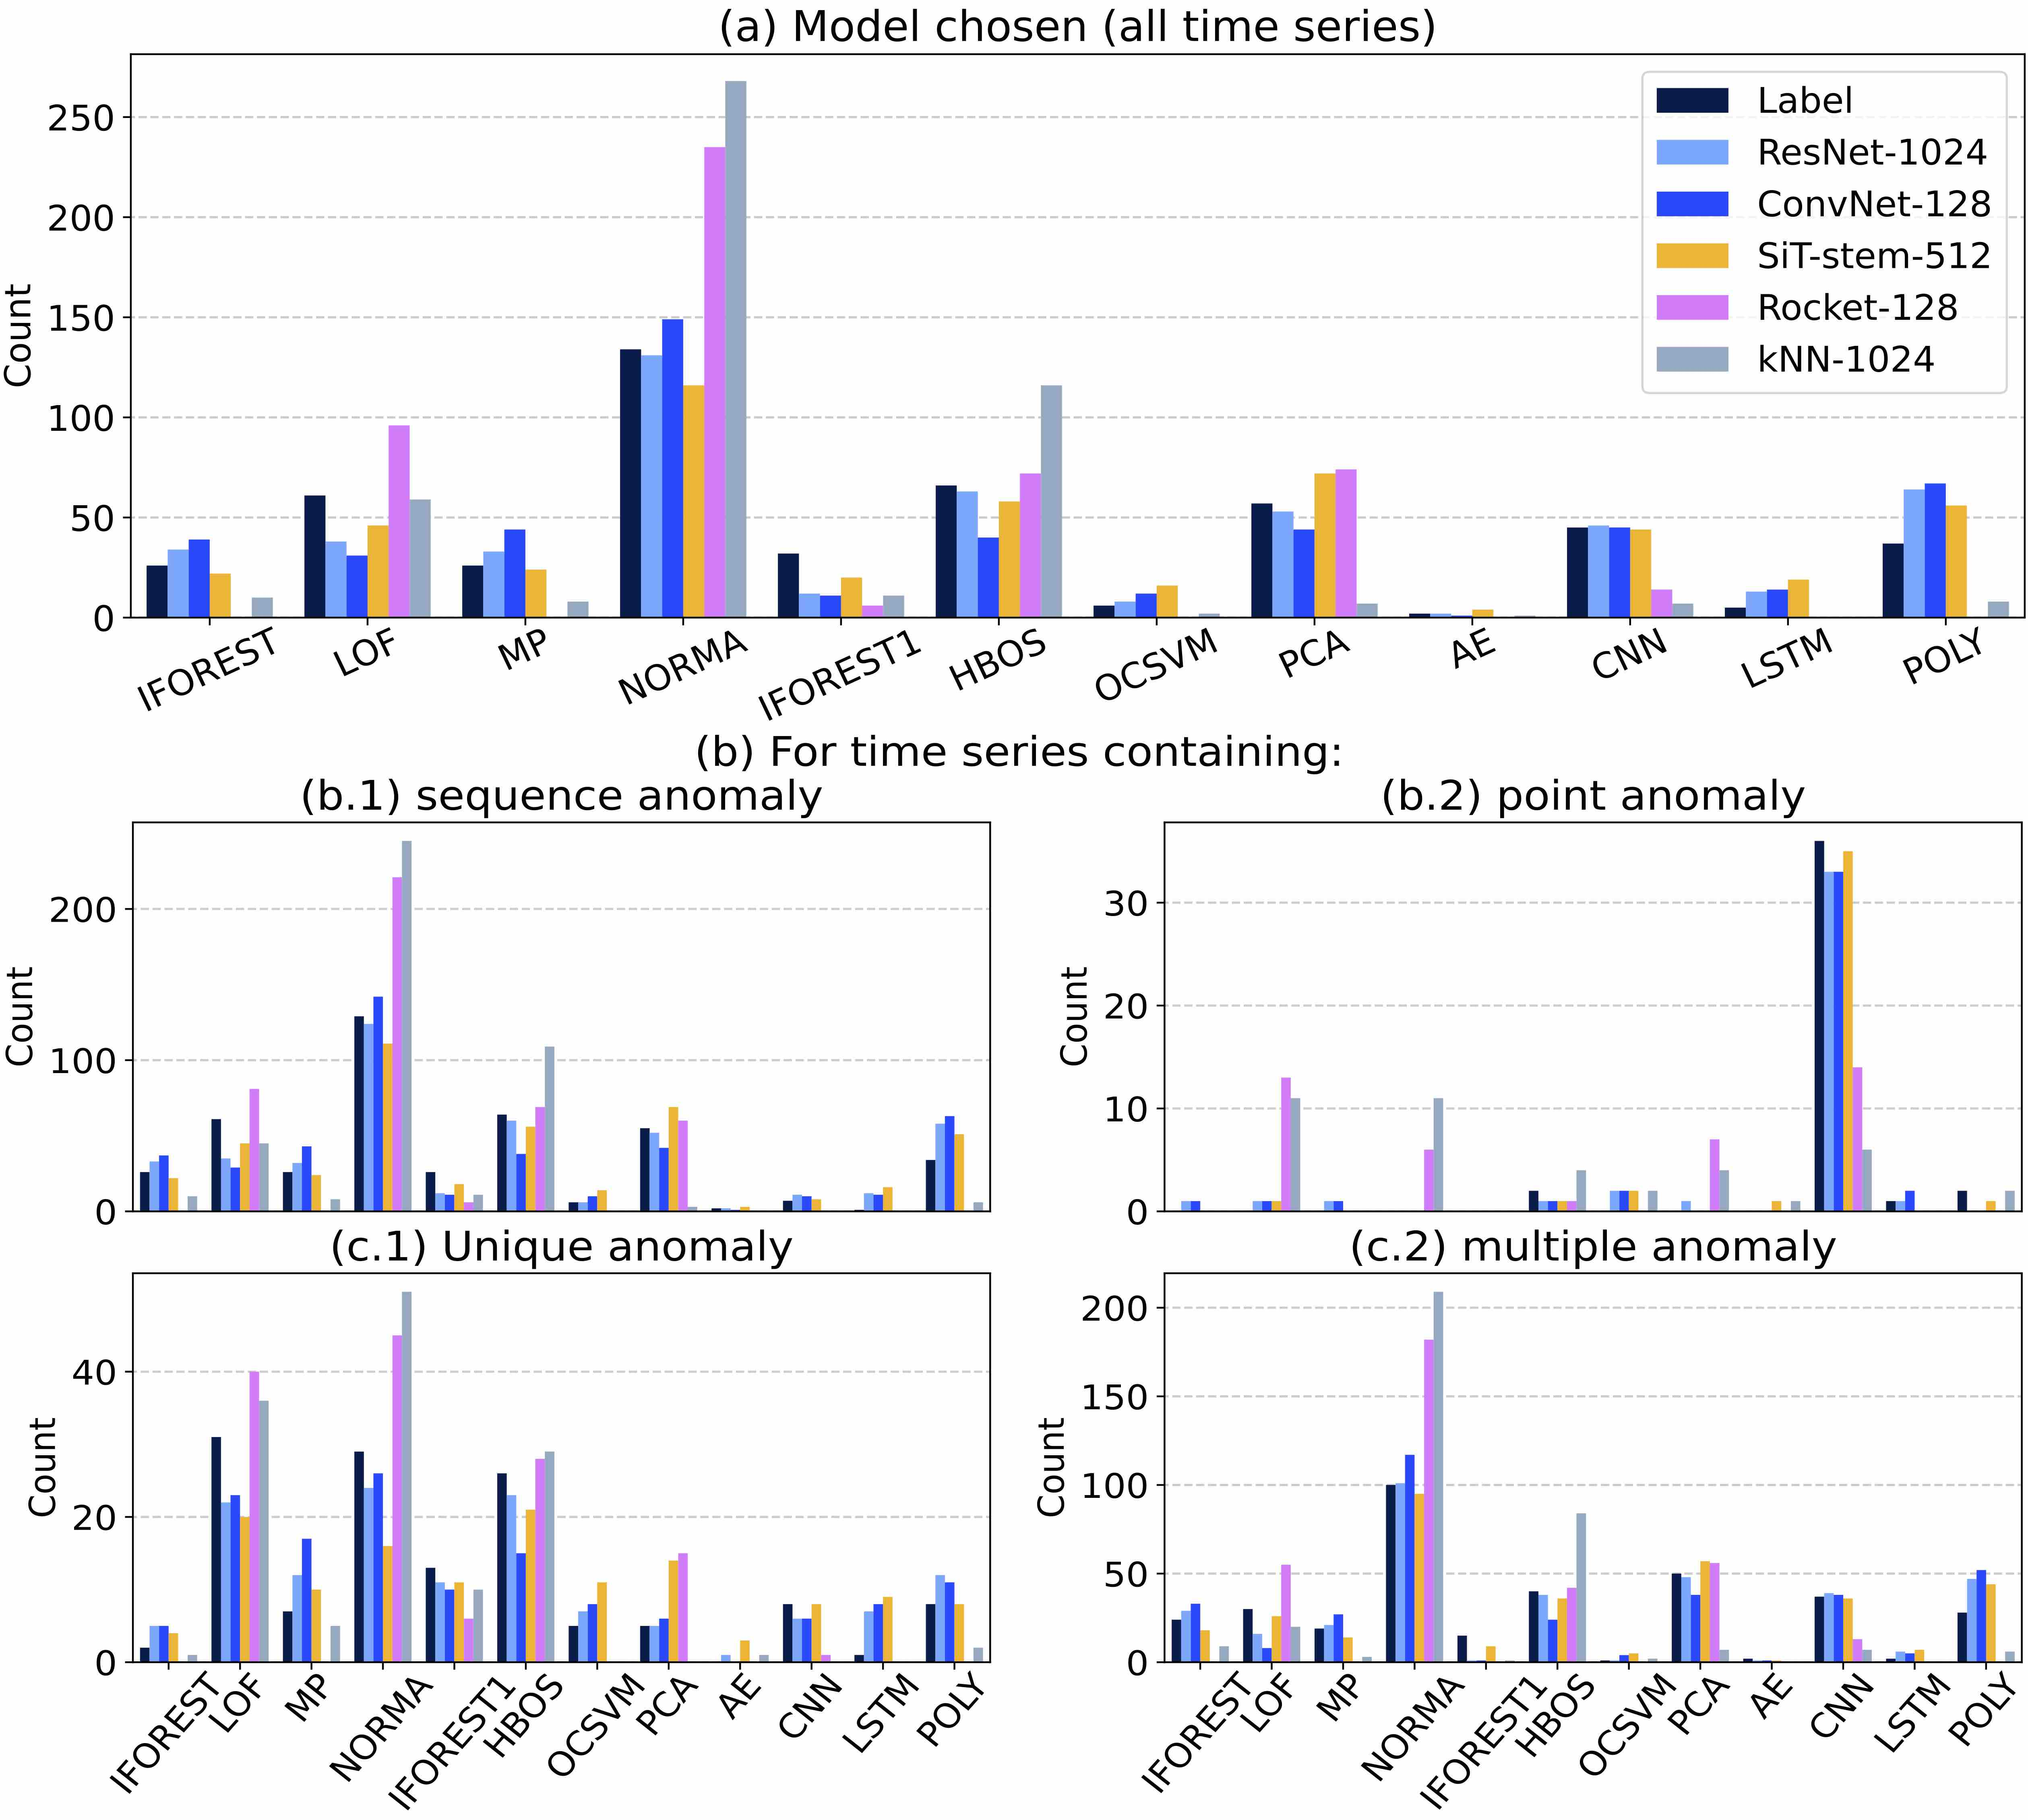
\includegraphics[width=\linewidth]{figures/Fig6.jpg}
        \caption{Distribution of the selected models for five models (the best for each category) compared to the distribution of the labels (in black). Difference of distributions between time series containing (b) sequence and point anomalies, and (c) unique or multiple anomalies.}
        \label{fig:classif_distrib}
\end{figure}

Figure~\ref{fig:overall_res} (a) depicts the overall VUS-PR over the entire TSB-UAD benchmark (i.e., each box-plot corresponds to 497 accuracy values for the 497 time series into the test set). The Convolutional-based approaches are in dark blue, the Transformer-based approaches are in yellow, the Feature-based approaches are in light blue, Rocket models are in violet, and the anomaly detection methods of the TSB-UAD benchmark are in light grey. The oracle is the top box plot (in white), and the Avg Ensemble is the orange box plot. The box-plot are sorted based on the median value. In total, we compare 142 models on 497 time series. In Figure~\ref{fig:overall_res}, we depict only the models with the window length that leads to the best VUS-PR.

First, almost all model selection methods outperform the existing anomaly detection methods. We also see that most model selection methods outperform the Avg Ensemble approach. Thus, we can conclude that model selection using time series classifiers significantly improves the state-of-the-art methods. 

More interestingly, we observe a partition in the ranking of the methods. First, Convolutional and Transformer-based approaches produce equivalent accuracy values and represent the top-48 methods. However, whereas all the Convolutional-based methods are in the top-48, a few of the Transformer-based approaches are further away in the ranking. Moreover, the first non-deep learning method is $rocket$-$128$ (ranked 49), followed closely by $knn$ models. We also observe that the $rocket$ approaches are very spread across the ranking ($rocket$-$128$ is ranked 50, and $rocket$-$16$ is ranked 124). This implies that the choice of window length strongly impacts accuracy. Overall, the best selection model is 2.8 times more accurate than the best anomaly detection method in TSB-UAD.

Then, we also note that all the model selection methods are significantly less accurate than the Oracle. For example, in Figure~\ref{fig:overall_res} (a), there is a gap of 0.2 VUS-PR between the Oracle and the best model selection method. Such a significant gap indicates a large margin of improvement for future work. We also note that all model selection approaches produce accuracy values between 0 and 1 (as shown by each box-plot in Figure~\ref{fig:overall_res} (a)). This is caused by the large heterogeneity of individual detectors' performances (for some datasets and time series, none of the detectors are accurate). This means that no model selection method is guaranteed to perform above a given accuracy value. Making model selection more stable and robust is essential for several use cases.


\begin{figure}
    \centering
    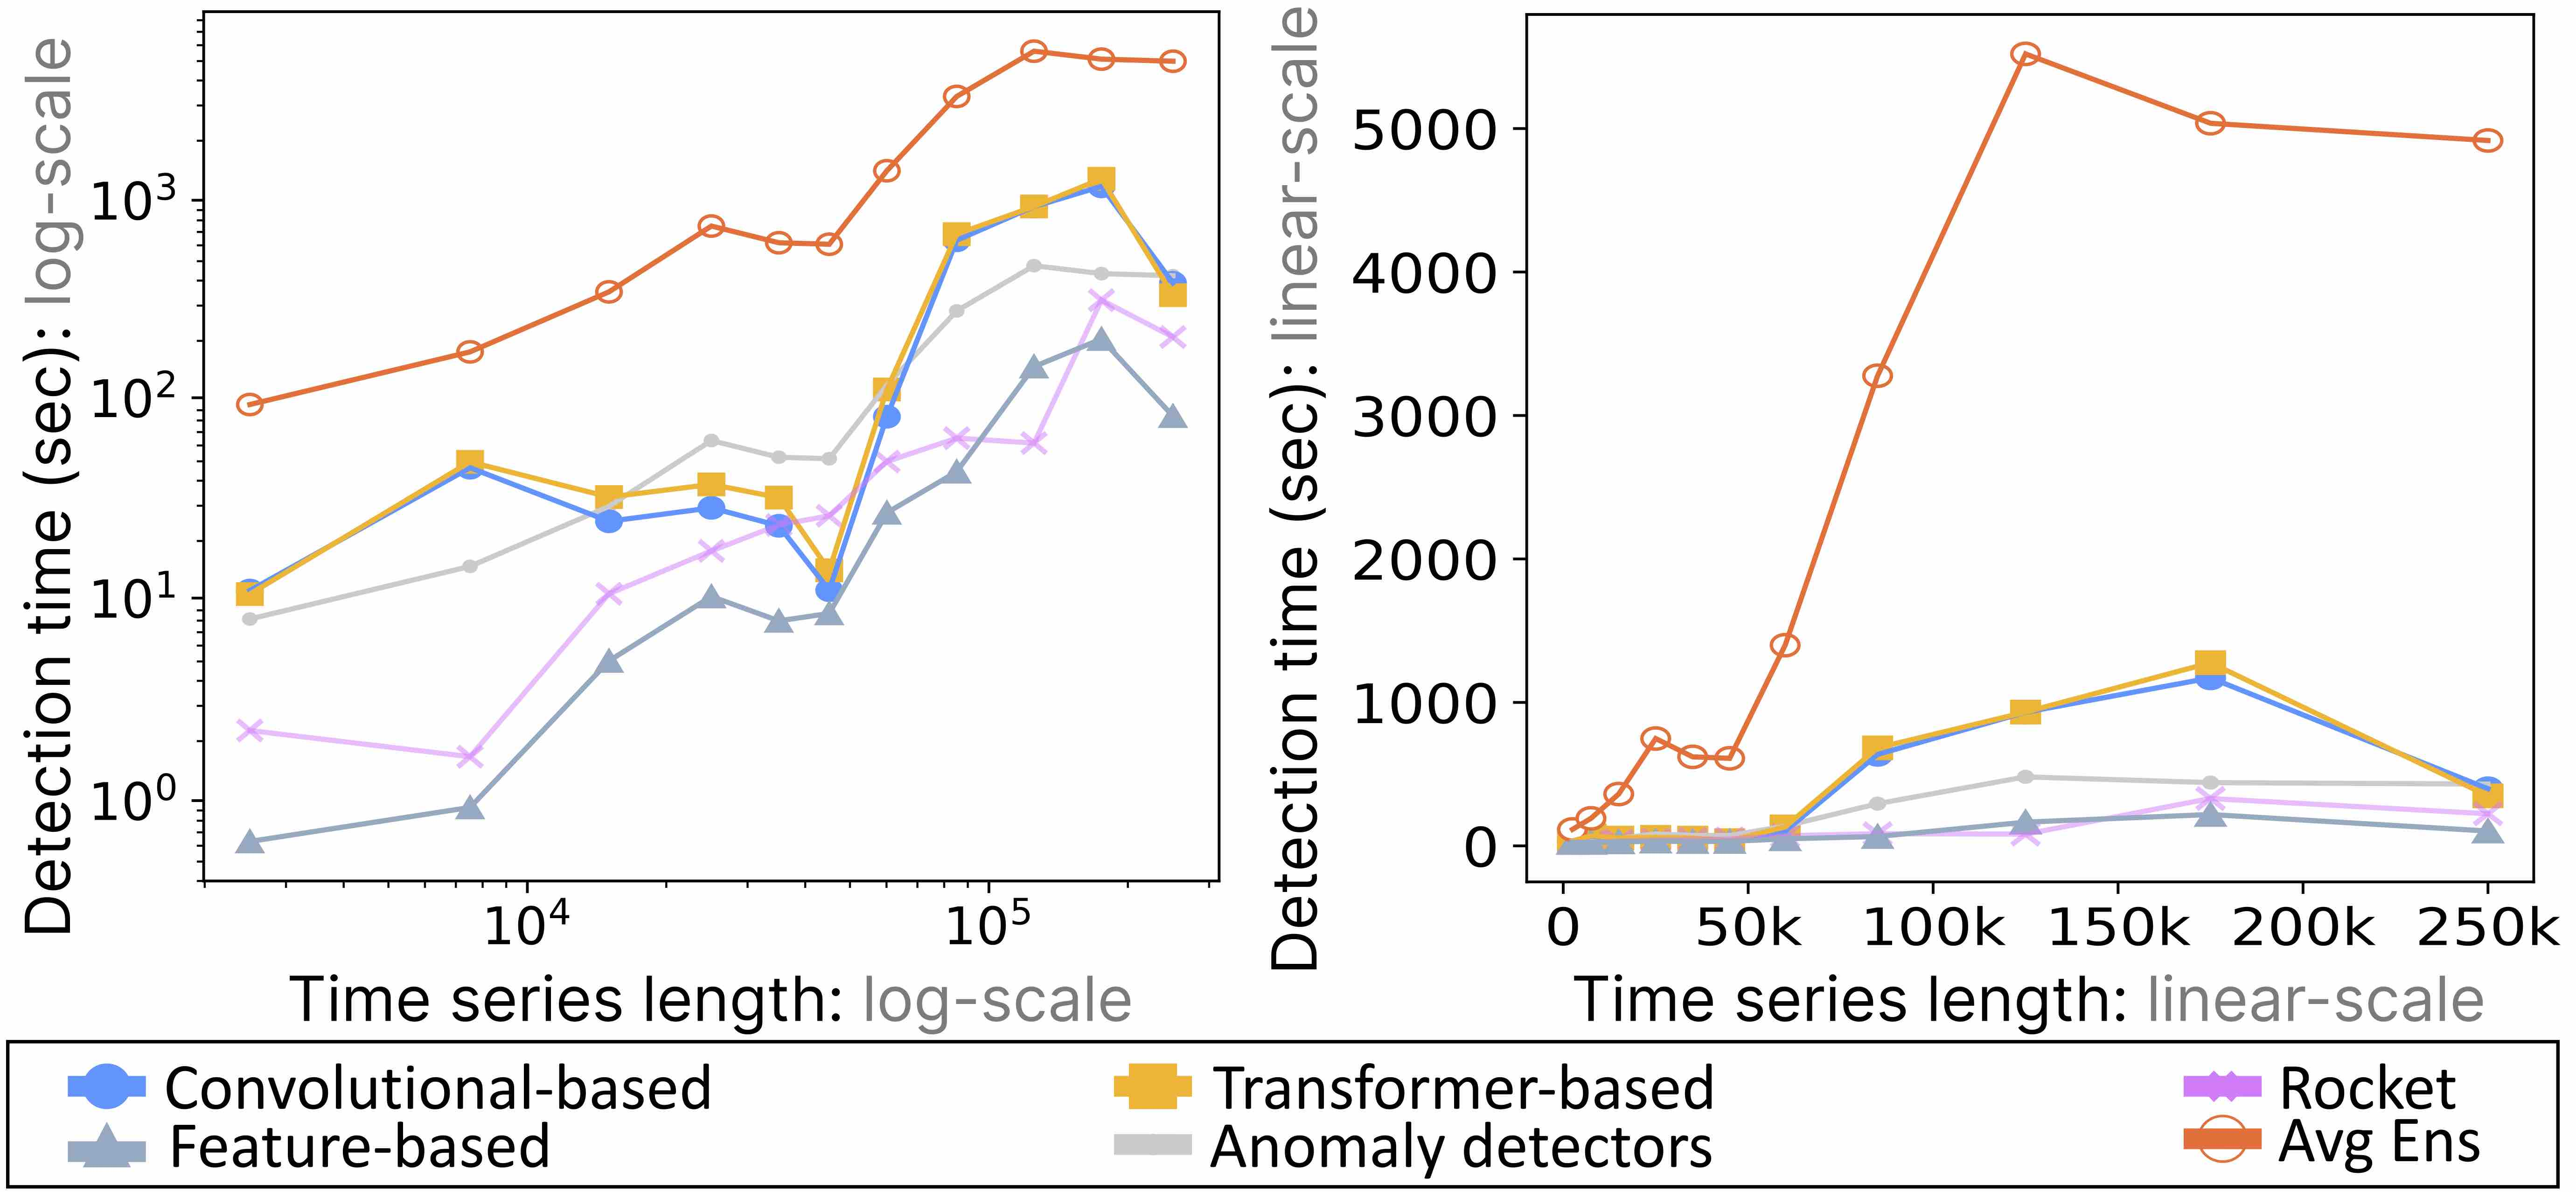
\includegraphics[width=\linewidth]{figures/Fig7.jpg}
        \caption{Execution time vs. length of model selection methods.}%for time series in TSB-UAD.}
        \label{fig:scalability}
\end{figure}

\subsubsection{\textbf{Model selected distribution}}
\label{exp:distribution}

We then inspect the prediction and the detector chosen by the model selection approaches. In this section, we consider only $resnet$-$1024$, $convnet$-$128$, $sit$-$stem$-$512$, $rocket$-$128$, and $knn$-$1024$. These approaches are the best models (using either AUC-PR or VUS-PR) based on the analysis conducted in Section~\ref{exp:overalleval} (you may find additional information on AUC-PR evaluation in our website~\cite{ourwebsite}).

Figure~\ref{fig:classif_distrib} (a) depicts the distribution of the chosen detectors by the 5 model selection approaches mentioned above for the entire TSB-UAD benchmark. The black bar corresponds to the true labels (i.e., the best detectors). We observe from Figure~\ref{fig:classif_distrib} (a) that $rocket$-$128$ and $knn$-$1024$ are significantly overestimating the detector NormA (as well as LOF for $rocket$-$128$ and HBOS for $knn$-$1024$), whereas $resnet$-$1024$, $convnet$-$128$, and $sit$-$stem$-$512$ are matching the correct distribution of detectors (we observe a slight underestimation of LOF, IFOREST1 and an overestimation for POLY).

Moreover, we measure the prediction distribution differences for time series containing sequence anomalies (Figure~\ref{fig:classif_distrib} (b.1)) and point anomalies (Figure~\ref{fig:classif_distrib} (b.2)), and for time series containing only one anomaly (Figure~\ref{fig:classif_distrib} (c.1)) and multiple anomalies (Figure~\ref{fig:classif_distrib} (c.1)). We first observe that predictions of model selection methods are significantly different for time series with sequence and point anomalies. More specifically, $resnet$-$1024$, $convnet$-$128$, and $sit$-$stem$-$512$ are correctly selecting the method CNN, whereas $rocket$-$128$ and $knn$-$1024$ are over selecting LOF and NormA for time series containing point anomalies. However, for sequence anomaly, as it represents most of the TSB-UAD benchmark, the prediction distribution is similar to the one over the entire benchmark. Moreover, the correct predictions of $resnet$-$1024$, $convnet$-$128$, and $sit$-$stem$-$512$ for time series containing point anomalies are interesting, as this information is not provided in the training step. Therefore, these models found discriminant features in the time series that indicate whether it might contain a point or a sequence anomaly.

We, finally, measure the differences between the prediction distribution of model selection methods between time series containing unique and multiple anomalies. The true labels (black bars in Figure~\ref{fig:classif_distrib} (c.1) and (c.2)) indicate that, for unique anomalies, the best detectors are LOF, NormA, and HBOS and for multiple anomalies, the best detector is NormA. We observe that all model selection approaches correctly select LOF, NormA, and HBOS for time series containing a unique anomaly. The latter indicates that model selection methods can extract discriminant features that indicate if one time series is more likely to have multiple anomalies.


\subsubsection{\textbf{Execution Time Evaluation}}

We now discuss the execution time of model selection methods. In this section, we focus only on the detection time (i.e., the number of seconds required by a method to predict the detector to use and to run it). Figure~\ref{fig:overall_res} (b) depicts the detection time (in log scale) for each method and detector in the TSB-UAD benchmark. We first observe that the Avg Ensemble required to run all detectors is significantly slower than the rest. Then, all model selection methods are of the same order of magnitude as the detectors. We also observe that all the deep learning methods are slower than the feature-based approaches. This is surprising because the detection time mainly depends on the chosen detector. Overall, we conclude that method selection is the only viable solution that outperforms the existing anomaly detection methods and can be executed in the same order of magnitude of time. Finally, we depict in Figure~\ref{fig:scalability} the scalability of model selection methods versus individual detectors and the Avg Ensemble approach when the time series length increases. We observe that, on average, the execution time of model selection approaches increases similarly to the execution time of individual detectors when the time series length increases. We also observe that the time series length significantly impacts the Avg Ensemble approach execution time. The latter shows the scalability issue of the Avg Ensemble approach for very large time series.

\begin{figure}
    \centering
    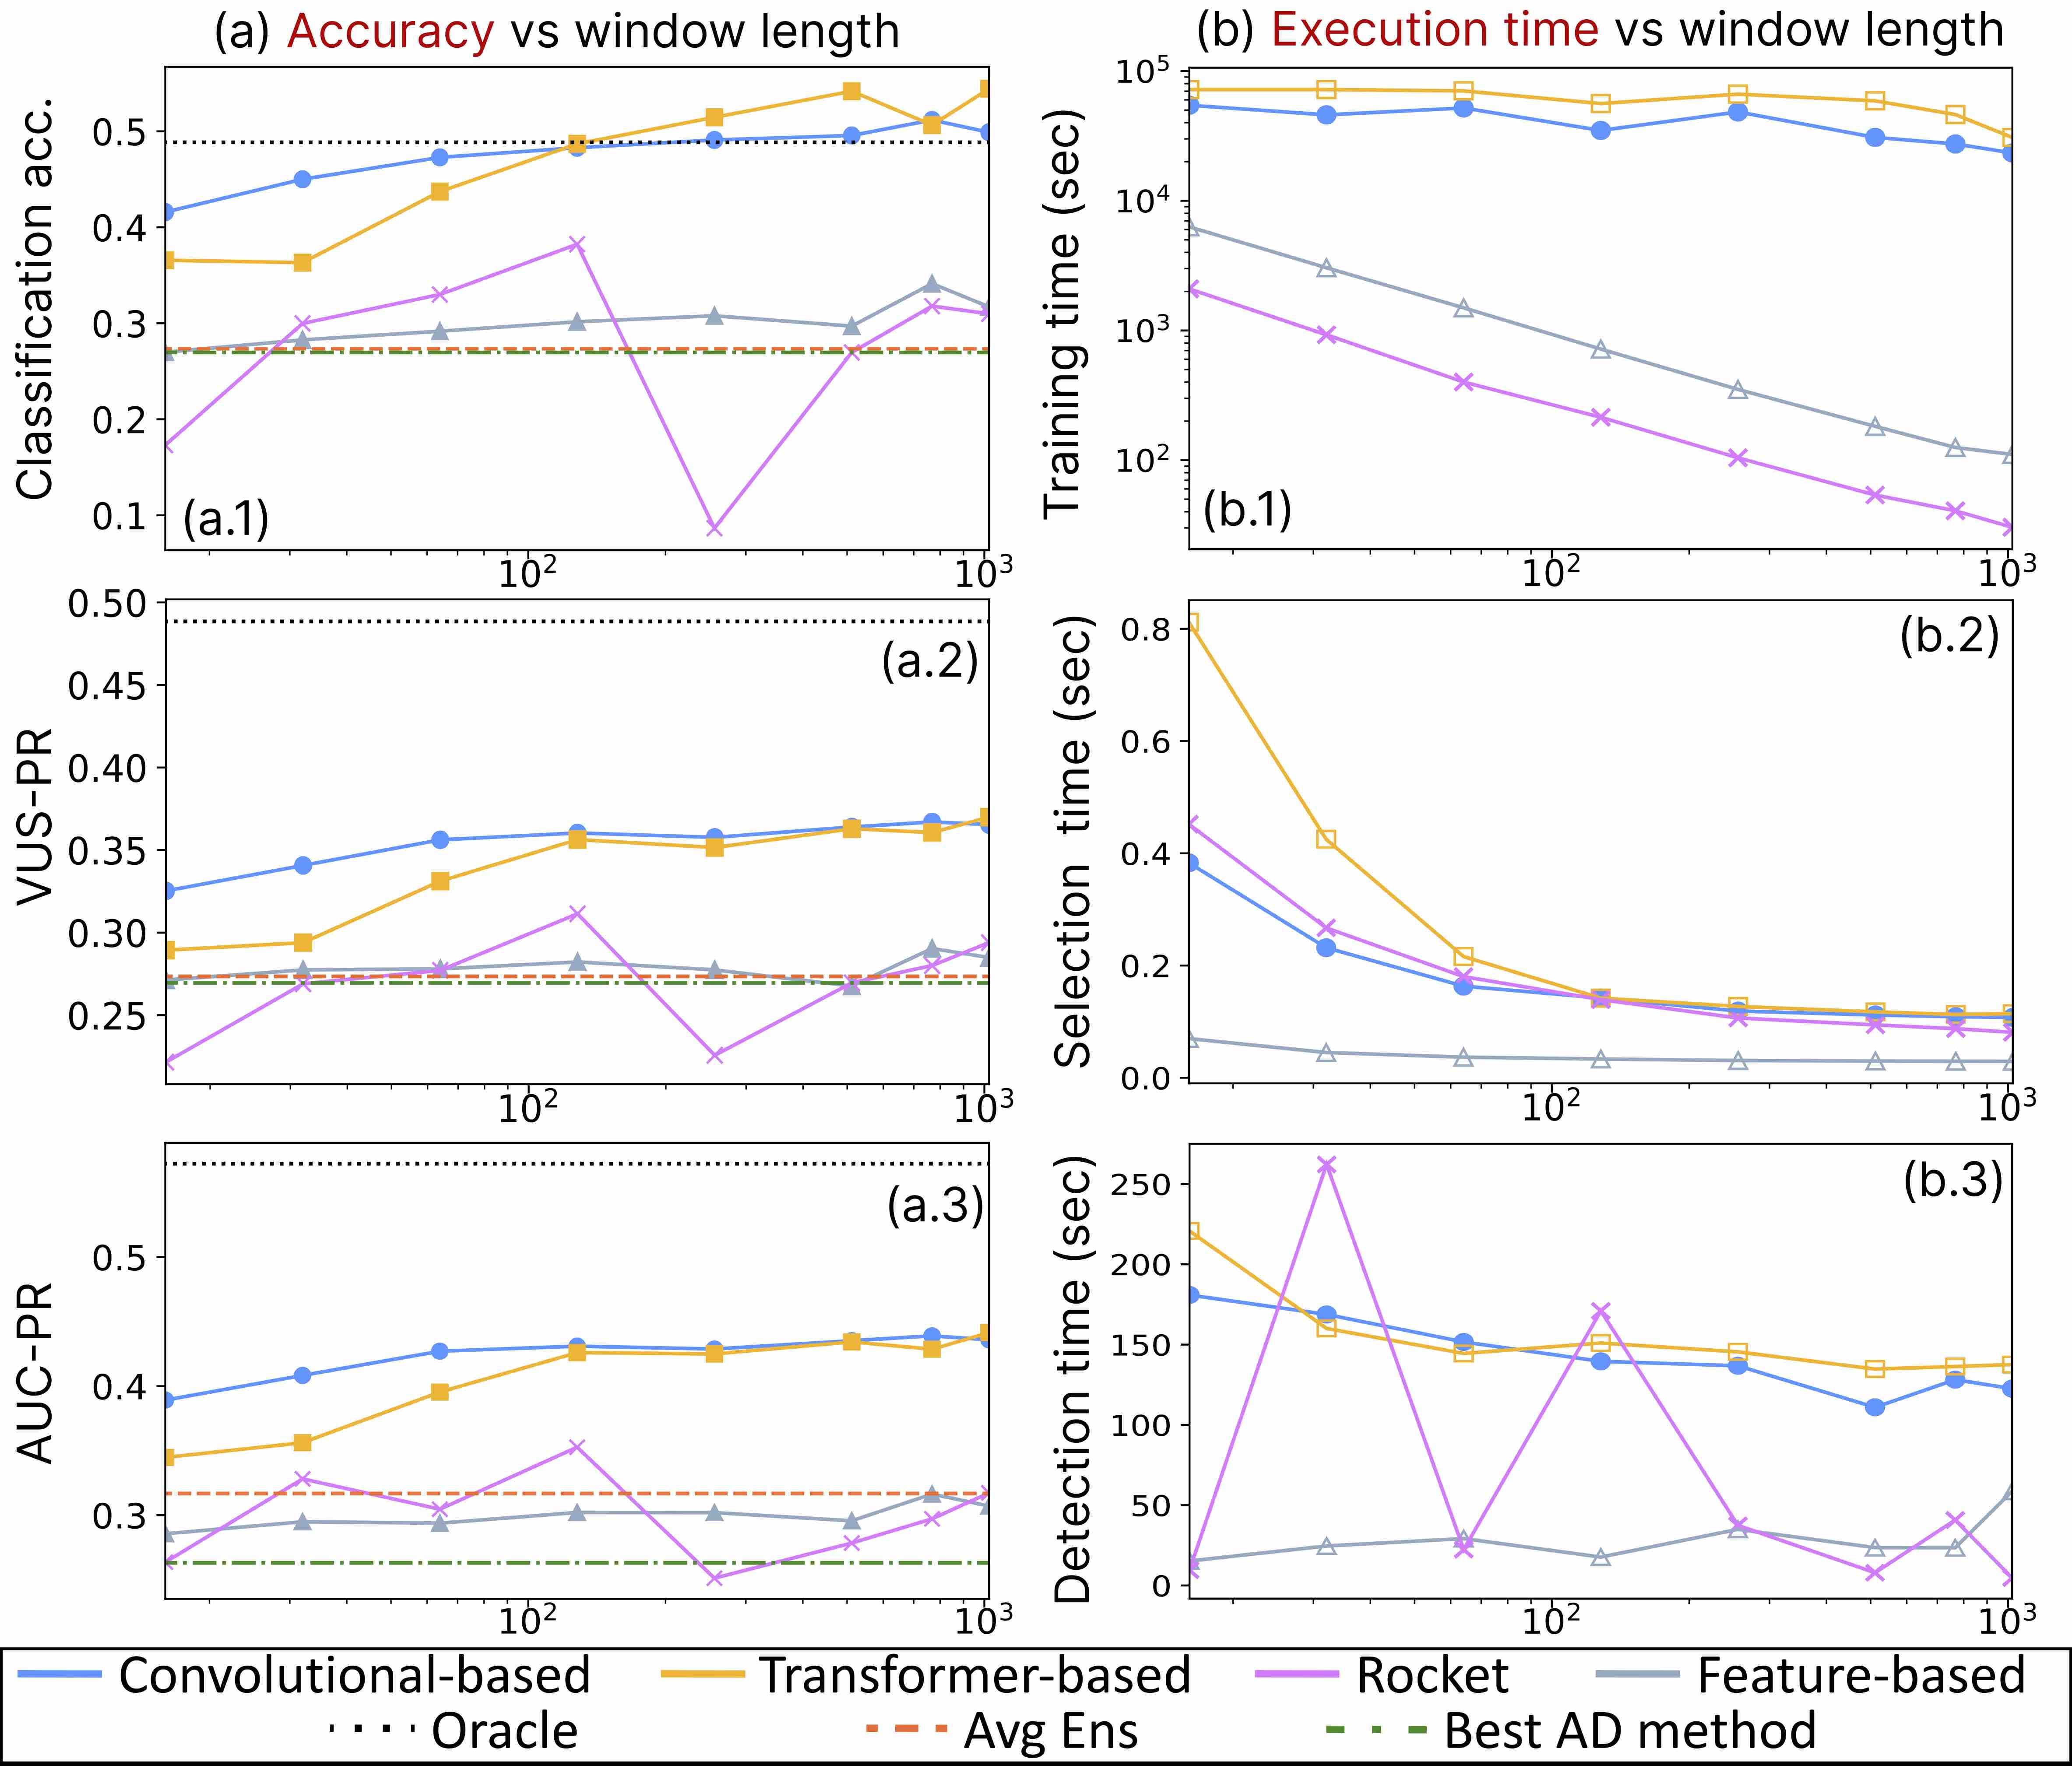
\includegraphics[width=\linewidth]{figures/Fig8.jpg}
        \caption{(a) Accuracy ((a.1) classification accuracy, (a.2) VUS-PR and (a.3) AUC-PR) and (b) execution time ((b.1) training time, (b.2) selection time and (b.3) detection time) versus window length $\ell$.}
        \label{fig:lengthinfl}
\end{figure}

\subsection{Influence of the Window Length}
\label{exp:windowlength}


In this section, we analyze the influence of the window length on classification accuracy (Figure~\ref{fig:lengthinfl} (a.1)), anomaly detection accuracy (Figure~\ref{fig:lengthinfl} (a.2) and (a.3)) and execution time (Figure~\ref{fig:lengthinfl} (b)). We perform the analysis per group of methods (i.e., average for Convolutional, Transformer, \journalv{Rocket}, and Feature-based methods).

We first observe in Figure~\ref{fig:lengthinfl} (a) that Convolutional-based and Transformer-based methods outperform the best anomaly detection methods (green dashed line in Figure~\ref{fig:lengthinfl} (a.2) and (a.3)), the Avg Ensemble approach (orange dotted line in Figure~\ref{fig:lengthinfl} (a.2) and (a.3)), Rocket and Feature-based methods, whatever the length used with regard to the classification accuracy, VUS-PR, and AUC-PR. We also observe that Transformer-based approaches are less accurate for shorter lengths (less than 100 points), whereas the accuracy of Convolutional-based approaches is stable regardless of the window length. Overall, Transformer and Convolutional-based approaches converge to the same anomaly detection accuracy (both for VUS-PR and AUC-PR) when the window length increases.

\begin{figure}
    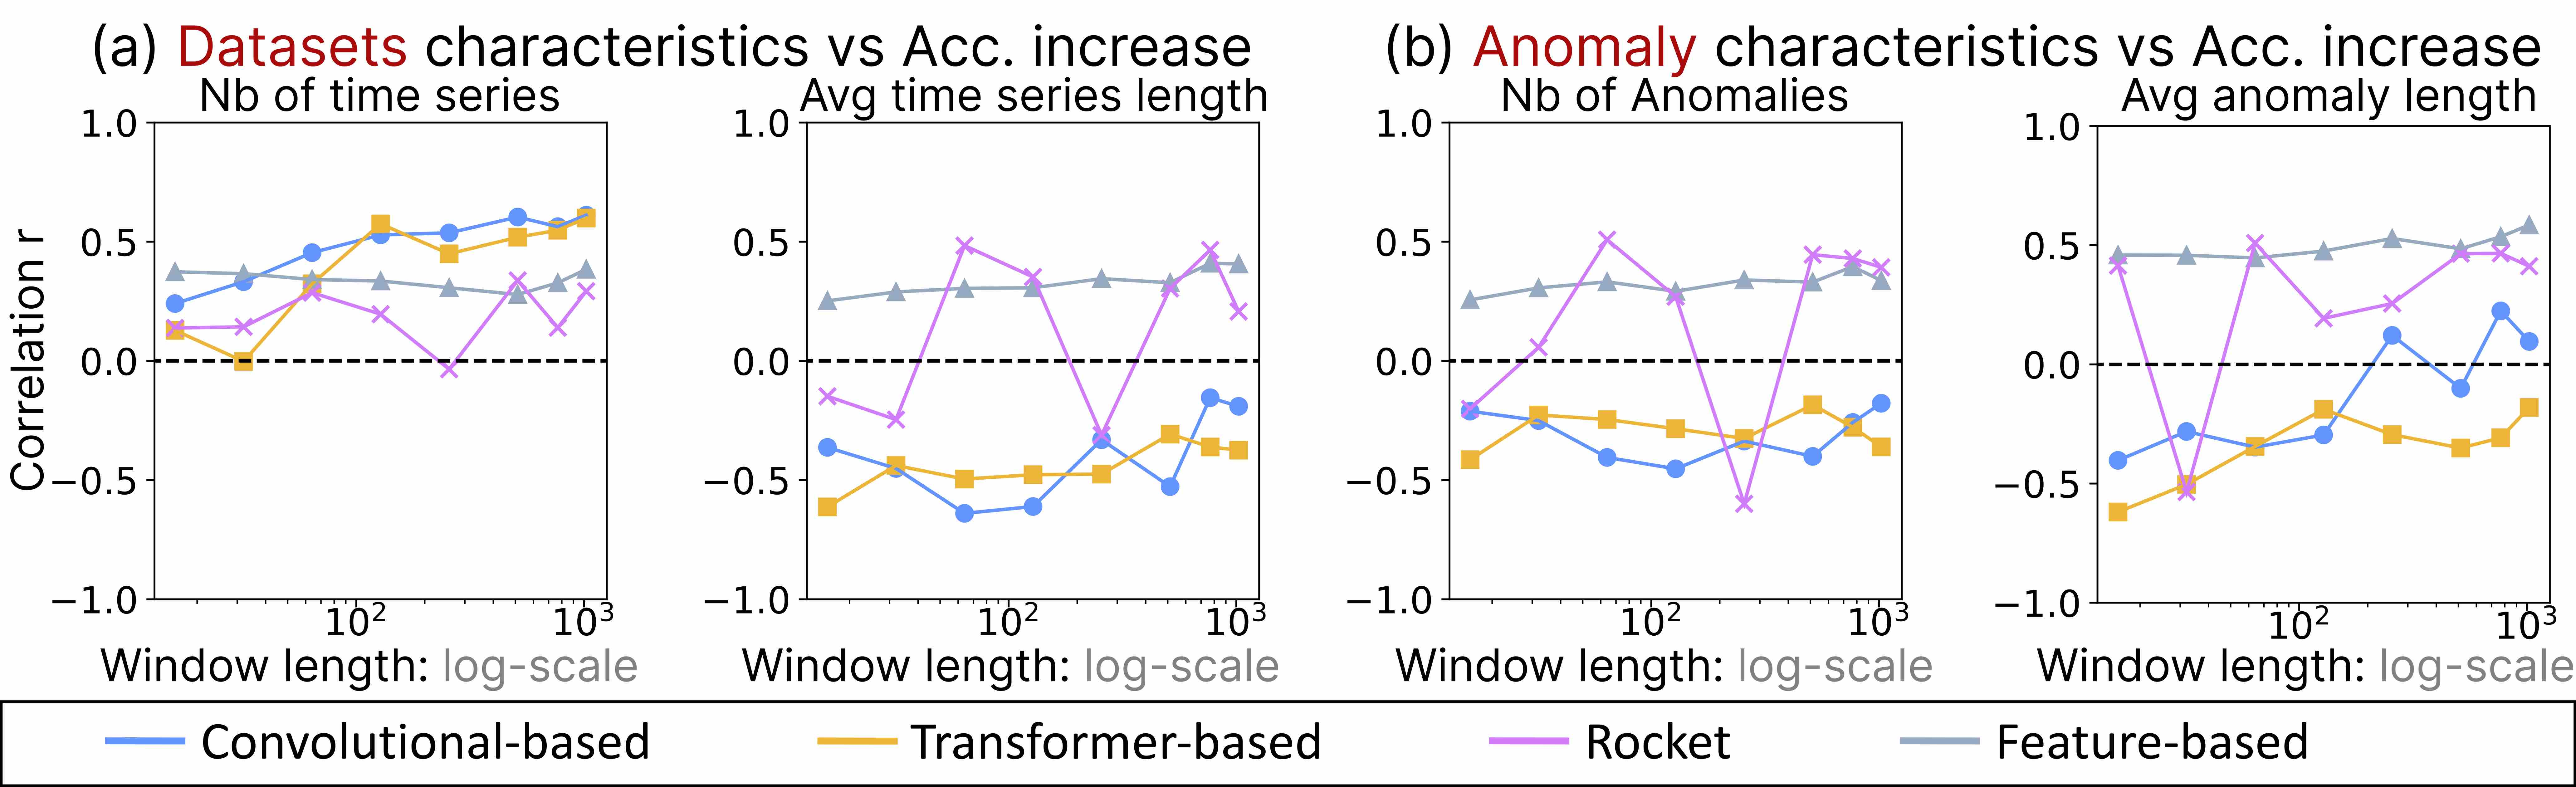
\includegraphics[width=\linewidth]{figures/Fig9.jpg}
    \caption{Correlation between accuracy and time series characteristics vs. the window length used to train the model selection methods.}
    \label{fig:infl_charac}
\end{figure}

Furthermore, we observe that both \journalv{Rocket} and Feature-based approaches are significantly faster to be trained than Convolutional and Transformer-based approaches (Figure~\ref{fig:lengthinfl} (b.1)). We make the same observation for selection time  ((Figure~\ref{fig:lengthinfl} (b.2))). For the detection time, we observe that \journalv{Rocket} execution time is very unstable when compared to the other approaches. The latter means that the choice of length strongly impacts the model selection performed by \journalv{Rocket}, leading to very diverse selection and execution times.

In the general case, we can make the following two statements: (i) \journalv{A large window length results in faster selection time for the model selection process and better accuracy for Convolutional and Transformer-based approaches.} (ii) Feature-based approaches are significantly faster but less accurate than Convolutional-based and Transformer based approaches, \journalv{regardless of} the window length used.


\subsection{Influence of Datasets and Anomaly Types}
\label{exp:datasets}

In this section, we evaluate the influence of datasets and anomaly characteristics on model selection accuracy. We perform the analysis per group of methods (i.e., average performances for Convolutional, Transformer, Rocket, and Feature-based methods).

For this experiment, we evaluate the dataset and anomaly characteristics (i.e., the number of time series, the average length of the time series, the average number of anomalies and the average anomaly length). Figure~\ref{fig:infl_charac} depicts these characteristics (x-axis) versus the average increase of accuracy (VUS-PR of the model selection method subtracted by VUS-PR of the best anomaly detection method for each dataset) for each model selection method using a given window length. For instance, if a point (one model selection method on one dataset) is positive (above the black dotted line), then this model is more accurate on the corresponding dataset than the best anomaly detection method selected on this same dataset. %Figure~\ref{fig:infl_charac} (1) shows a specific example for window length $\ell=1024$. Figure~\ref{fig:infl_charac} (2) shows the correlation values (trend of the different lines in Figure~\ref{fig:infl_charac} (1)) versus the window length.
We generally observe low correlations between dataset and anomaly characteristics (i.e., $-0.6<r<0.6$). With such correlation values, we cannot conclude any factual statement on the impact of these characteristics and the model selection methods' performances. However, we can make the following observations.

%First, Figure~\ref{fig:intro_fig} (a.1) shows that all model selection methods (with a window length $\ell=1024$) are more likely to be accurate on large datasets. 
First, Figure~\ref{fig:infl_charac} (a) shows that the number of time series is impacting more substantially Convolutional and Transformer-based approaches with large window lengths. For the average time series length, only Feature-based approaches are positively impacted. On the contrary, Convolutional and Transformer-based approaches are less accurate when the average time series length is increasing. These observations imply that Convolutional and Transformer-based are more affected by the number of examples in the dataset rather than the length of each instance. In contrast, Feature-based approaches benefit from both more and large instances.

Then, Figure~\ref{fig:infl_charac} (b) shows that Feature-based approach accuracy is increasing with the anomaly characteristics, whereas these characteristics either do not or negatively impact Convolutional and Transformer-based methods. More specifically, we observe that Feature-based approaches (regardless of the window length) are more accurate with time series containing large anomalies, and Convolutional-based approaches are less accurate (irrespective of the window length) when the number of anomalies increases.

We note that Rocket's correlation with the dataset and the anomaly characteristics is unstable. The latter is explained by the fact that the model prediction of Rocket is very sensitive to the window length (as described in Section~\ref{exp:windowlength}). Thus, it is impossible to make a conclusion on Rocket's performances, datasets, and anomalies.


\subsection{Detection vs Classification Accuracy}
\label{exp:detectionvsclass}

In this section, we analyze the relationship between the model selection methods' classification accuracy and the resulting anomaly detection accuracy. In this experiment, we consider VUS-PR as anomaly detection measures. For this experiment, we extend the definition of $Oracle$ (introduced in Section~\ref{sec:problem_def}) as follows:

\begin{definition}
    We define $Oracle_{k,j}$ as a hypothetical model selection method that has a classification accuracy of $k \in [0,1]$ and selects the $j^{th}$ best detector (among $m$ detectors) in cases of misclassification. Thus, $Oracle_{1,1}$ always selects the best detector, and $Oracle_{0,m}$ always selects the worst detector. Finally, we define $Oracle_{k,R}$ as the model selection method with a classification accuracy of $k \in [0,1]$ and that randomly selects a detector in misclassification cases.
    \end{definition}

\begin{figure}
    \centering
    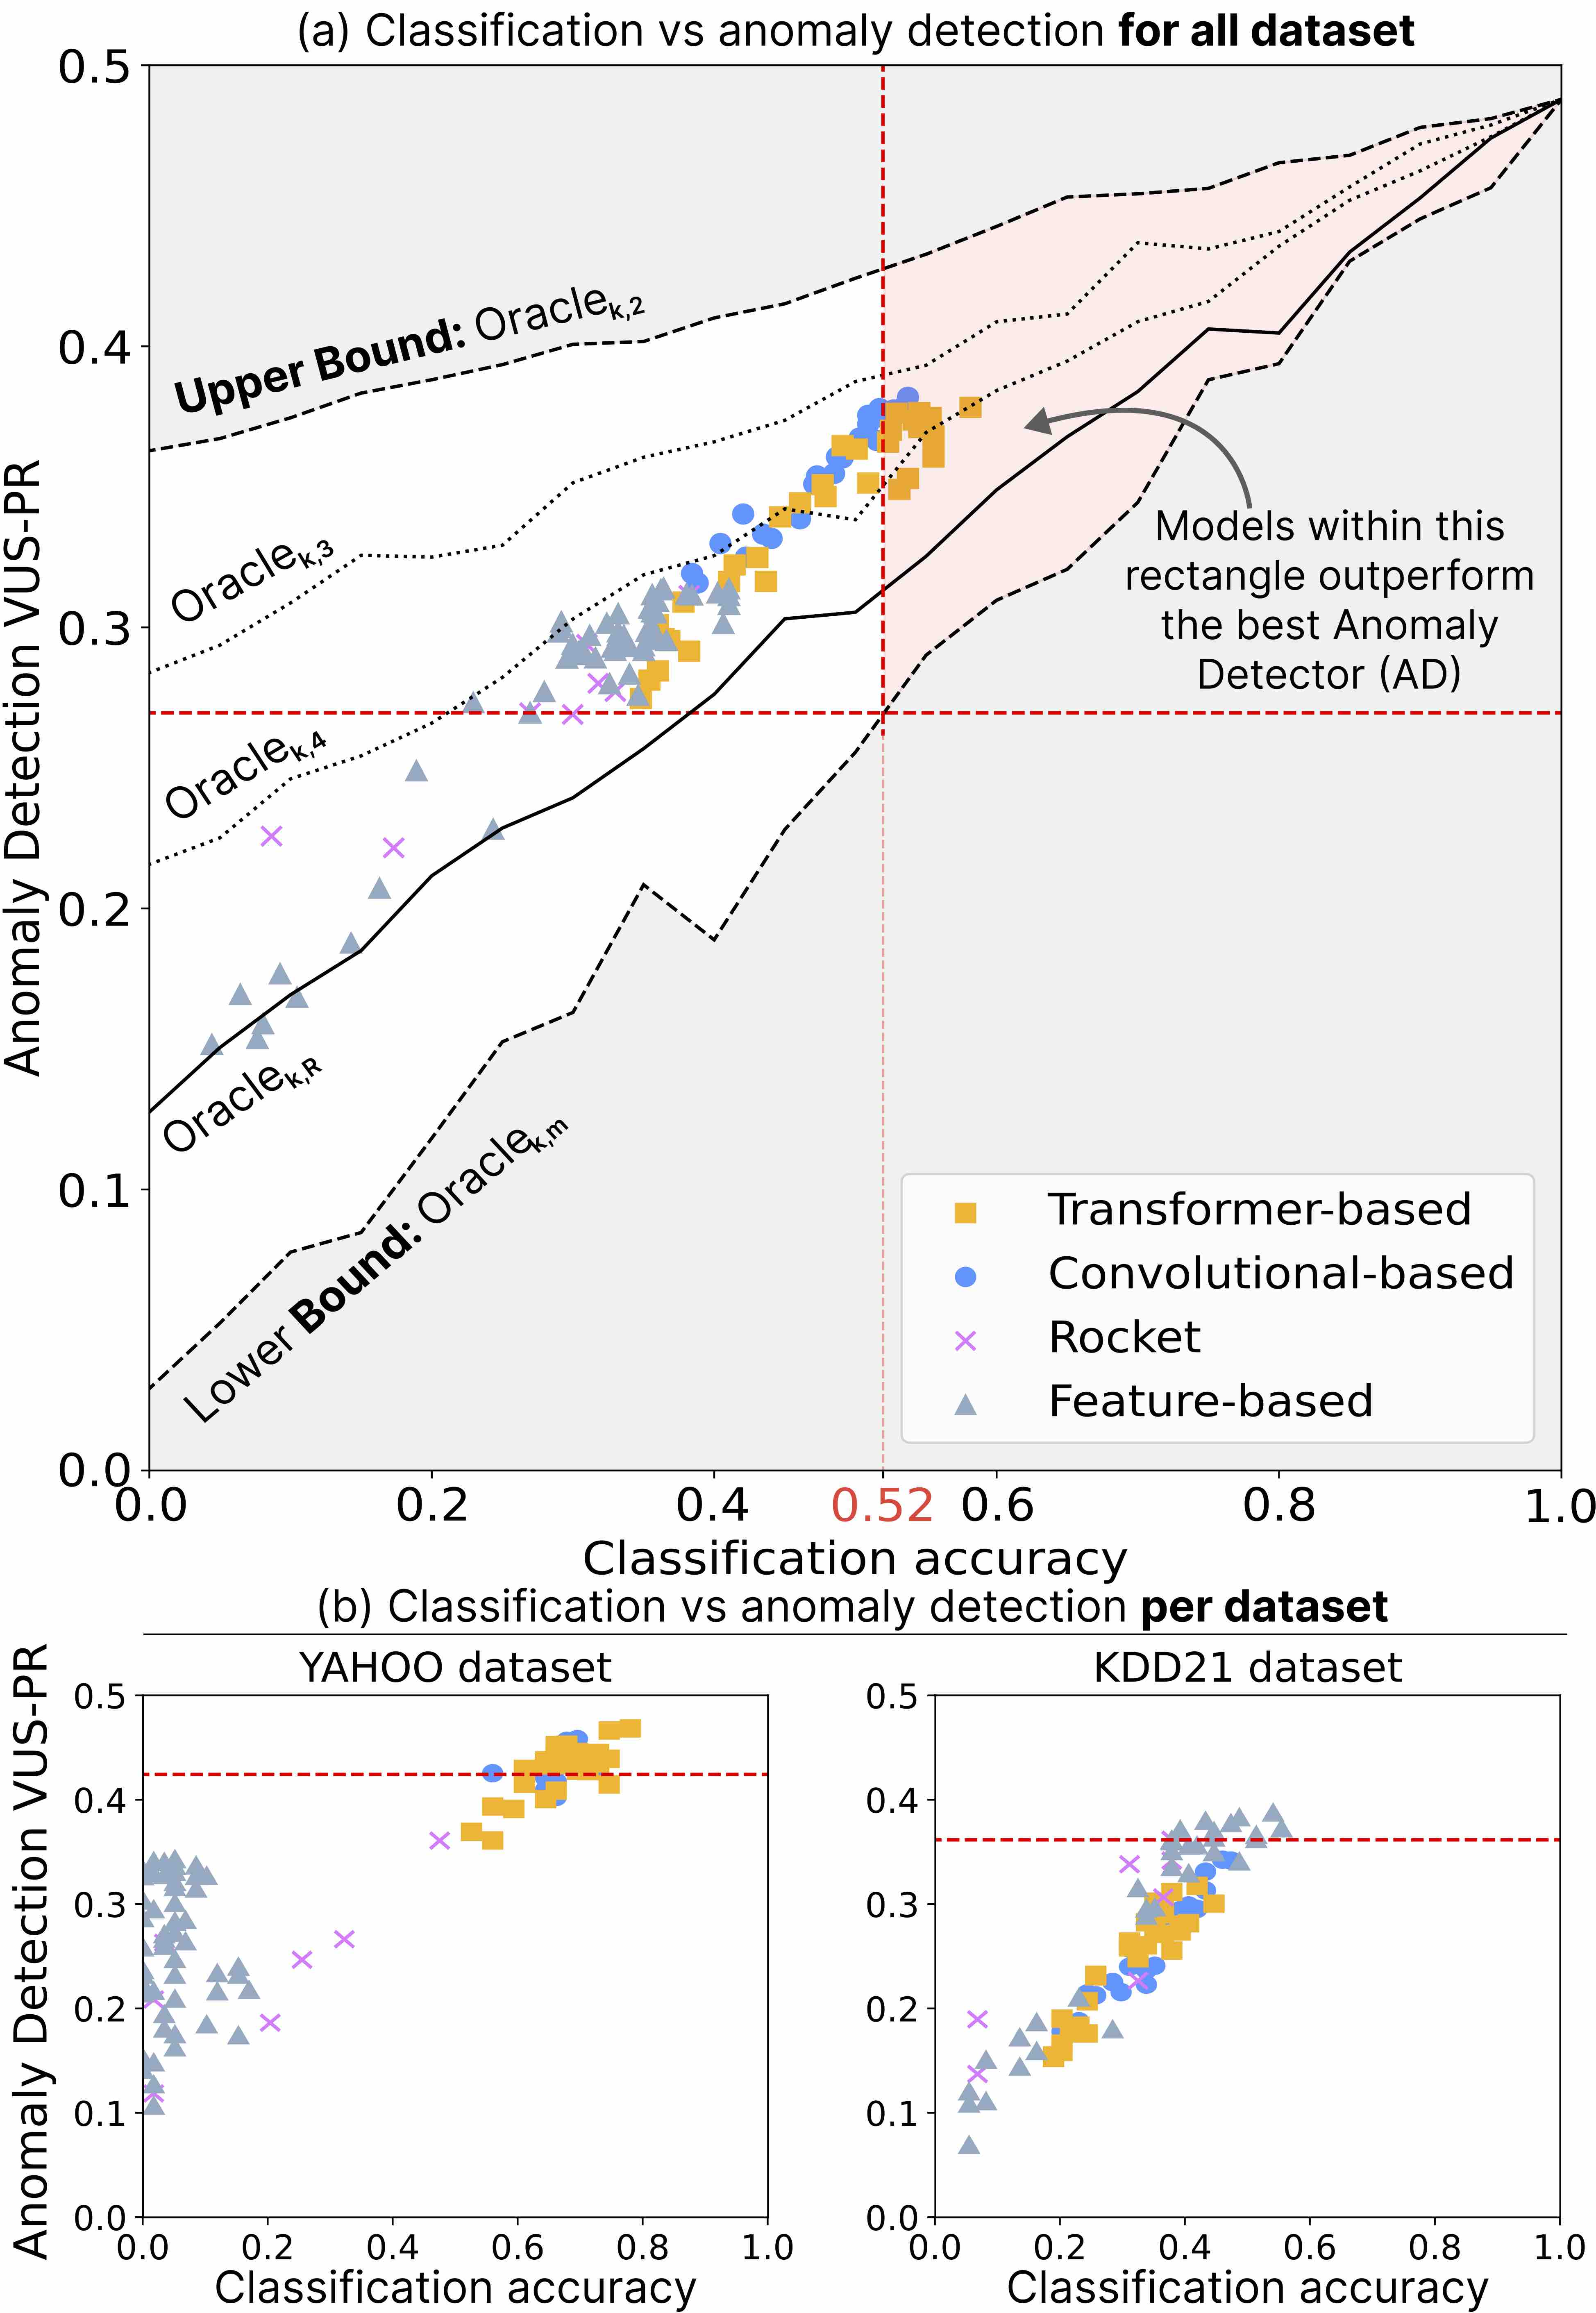
\includegraphics[width=\linewidth]{figures/Fig10.jpg}
        \caption{Classification accuracy versus anomaly detection accuracy (VUS-PR) for (a) all datasets and (b) two specific datasets.}
        \label{fig:class_AD}
\end{figure}


\begin{figure*}
    \centering
    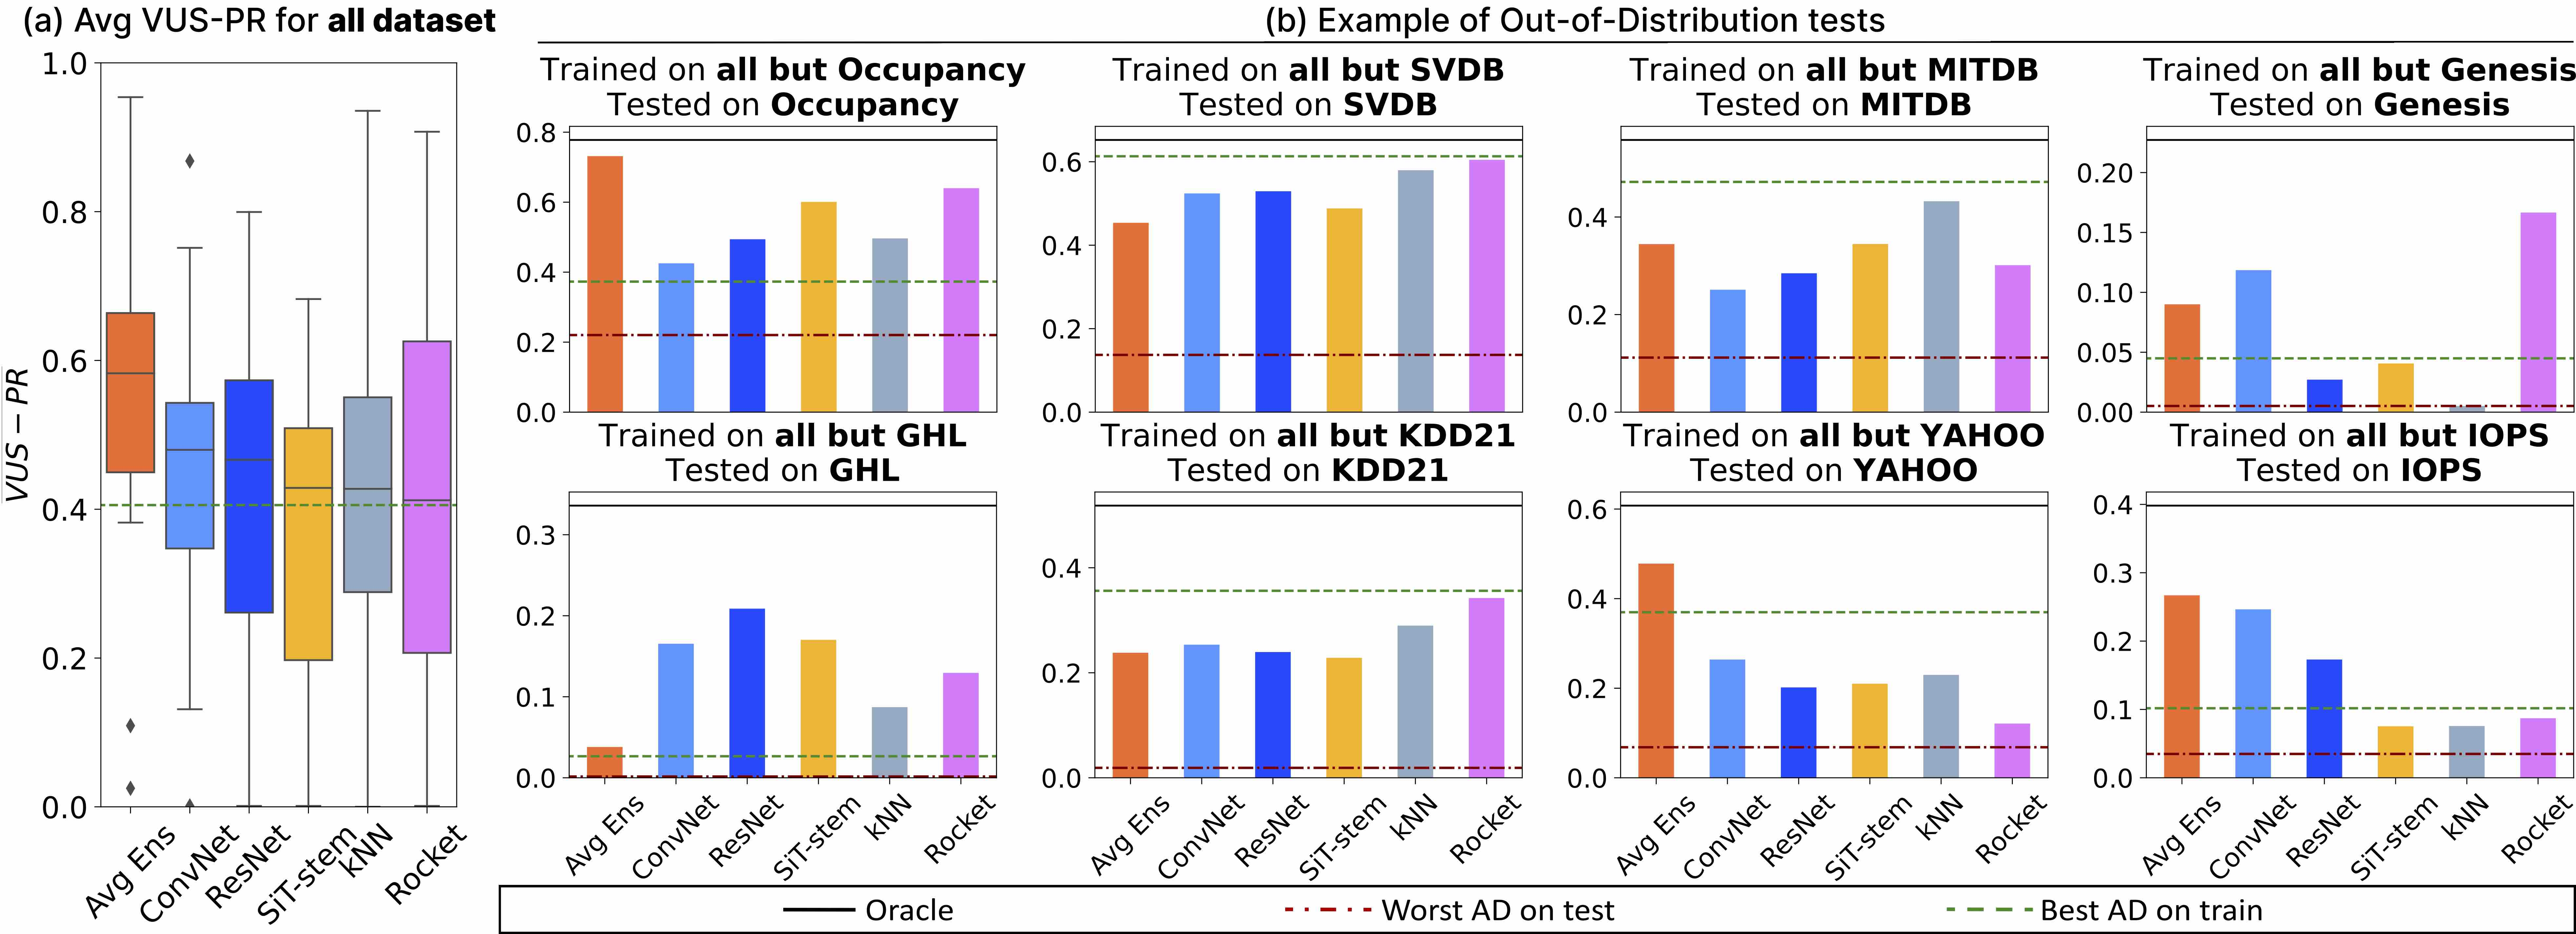
\includegraphics[width=\linewidth]{figures/Fig11.jpg}
        \caption{Out-of-distribution experiment, when model selection algorithms are trained on all but one dataset. (a) results for each dataset (when not included in the training set) and (b) average results.
    }
        \label{fig:one_vs_all}
\end{figure*}

Figure~\ref{fig:class_AD} depicts the latter comparison for all datasets (Figure~\ref{fig:class_AD} (a)), and two specific datasets (Figure~\ref{fig:class_AD} (b)). We first observe a strong correlation between classification accuracy and anomaly detection accuracy for each specific dataset and, on average, all datasets. However, methods belonging to different families (e.g., Feature-based or Transformer-based) are not performing the same. For instance, Figure~\ref{fig:class_AD} (a) shows that Feature-based approaches are not accurate for YAHOO but are the best models for KDD21. Overall, we observe that Convolutional and Transformer-based are more accurate in classification and anomaly detection (Figure~\ref{fig:class_AD}(b)). 

We also depict in Figure~\ref{fig:class_AD} (a) the lines corresponding to $Oracle_{k,2}$, $Oracle_{k,3}$, $Oracle_{k,4}$, $Oracle_{k,R}$, and $Oracle_{k,m}$. For a given classification accuracy, $k$, $Oracle_{k,2}$, and $Oracle_{k,m}$ correspond to the upper and lower bounds. The latter means that model selection approaches with a given classification accuracy will be within the previously mentioned upper and lower bounds for VUS-PR (i.e., in the grey zone in Figure~\ref{fig:class_AD} (a)). Thus, any model selection method that has a classification accuracy above 0.53 (intersection between the two dashed red lines) is better than the current best anomaly detection method in TSB-UAD (i.e., red dashed line in Figure~\ref{fig:class_AD} (b)). 
This is true only for a few Convolutional- and Transformer-based methods in our experiments.

Moreover, we compare the positions of the model selection methods with regard the $Oracle_{k,3}$, $Oracle_{k,4}$, and $Oracle_{k,R}$. We observe in Figure~\ref{fig:class_AD} (b) that almost all methods are above $Oracle_{k,R}$. The latter means that the model selection methods do not randomly select detectors when the wrong detector is selected. Moreover, most models follow the $Oracle_{k,4}$ line. The latter indicates that the models averagely select the third-best in case of misclassification. Finally, the observations discussed above demonstrate three important statements: (i) classification accuracy can be used as a proxy for anomaly detection accuracy, and without computing the anomaly detection accuracy, we can provide an anomaly detection accuracy lower and upper bounds; (ii) the gap between the best model selection and the top right corner of the grey zone shows that there is a significant margin for improvement for future work; (iii) the vertical gap between the models and the upper bound ($Oracle_{k,2}$) shows that there is an important margin of improvement in the prediction rank: a model with the same classification accuracy can gain up to $0.1$ VUS-PR if it better selects models.


\subsection{Out-of-Distribution Experiments}
\label{exp:sup2unsup}

At this point, we tested the performances of the model selection methods when trained on a subset of the benchmark with examples from all 16 datasets available. \journalv{These results are interesting when we suppose that a user wants to analyze datasets similar to the one considered in the benchmark.} In some cases, though, we may want to analyze time series that are not similar to any of those in the benchmark. Therefore, in this section, we measure the ability of the model selection methods to be used in an unsupervised manner (i.e., used for datasets that are not similar to the one used in the training set). We run the following experiment. We train the model selection methods on 15 datasets (70\% of the time series for training and the other 30\% for validation), and we test on the remaining one. We try all 16 possible test partitions, and (for brevity) report 8 of these tests in Figure~\ref{fig:one_vs_all} (a). We only show the results for the best-performing model selection methods listed in Section~\ref{exp:distribution}\journalv{, namely, $resnet$-$1024$, $convnet$-$128$, $sit$-$stem$-$512$, $rocket$-$128$, $knn$-$1024$ and the Averaging ensemble for comparison. For simplicity, we only report the model's name without the window length.}

Figure~\ref{fig:one_vs_all} (a) \journalv{illustrates} the normalized VUS-PR (\journalv{denoted} $\overline{VUS\text{-}PR}$) for all 16 tests: \journalv{$\overline{VUS\text{-}PR}$} of 1 corresponds to the VUS-PR of the \emph{Oracle} on each test, while 0 corresponds to the worst anomaly detection methods on each test. This figure shows that, in the unsupervised case, the Avg Ensemble outperforms all model selection methods, as well as the best anomaly detection method based on the accuracy performance measured on the train set (dotted green line in Figure~\ref{fig:one_vs_all} (a)). The latter means that, for unknown datasets, it is safer to run all existing anomaly detection methods and average their scores. Knowing that such ensembling methods are not scalable (as shown in Figure~\ref{fig:overall_res}), Figure~\ref{fig:one_vs_all} (a) shows that ConvNet or ResNet is still a better choice than choosing the best anomaly detection method selected on train data (i.e., known data). However, kNN, Rocket, and SiT-stem are only slightly more accurate than the best anomaly detection method.

Figure~\ref{fig:one_vs_all} (b) depicts the average accuracy for 8 out of the 16 tests \journalv{(datasets excluded from the training set and used for testing)}. We observe very different results. First, for Electrocardiograms (SVDB), \journalv{neither} the model selection methods \journalv{nor} the Avg. Ensemble outperform the best anomaly detection method (selected on the training set). \journalv{However, for various kinds of sensor data (GHL and Occuopancy), model selection methods and the Avg Ensemble do outperform the best anomaly detection method (again selected on the training set).}  \journalv{This difference} can be explained by the fact that ECGs exhibit less \journalv{diverse} behaviors (i.e., repetitive normal patterns and similar anomalies) than other sensor data. \journalv{Consequently,} it is more likely to have one method in the benchmark that performs well on all \journalv{ECG} time series. \journalv{This observation is supported by the fact that the performance of the best anomaly detection method closely matches that of the Oracle for SVDB.}

These observations lead to the following remarks: (i) there is a significant margin of improvement when using the existing time series classifiers as model selection methods in the unsupervised case; (ii) when a new dataset arrives, it is safer in the general case to use an ensembling method such as the simple average of all anomaly scores; and (iii) for heterogeneous datasets (without known and repetitive normal or abnormal patterns), classifiers as model selection (mainly convolutional-based classifiers) can be used even though similar time series are not in the training set.
\section{Conclusions}
\label{sec:conclusions}

Time series anomaly detection is a challenging problem and an important area of research with many applications \journalv{ in many scientific, societal, and industrial domains.} Despite the multitude of solutions proposed in the literature, we observe that there exists no method that outperforms all others when measured on large heterogeneous benchmarks. Based on our experimental evaluation\journalv{, we answer the questions of Section~\ref{sec:objective} as follows:}

\begin{enumerate}%[noitemsep, topsep=0pt, parsep=0pt, partopsep=0pt, leftmargin=0.5cm]
	\item \textbf{Classification as Model selection}: We observe that time series classification methods accurately select anomaly detection models. Overall, Transformer and Convolutional-based model selection methods outperform each individual detector. Nevertheless, there is a large gap between the best method and the $Oracle$, motivating future work toward that direction.
	\item \textbf{Ensembling or selecting}: We observe that model selection is significantly more accurate than the Ensembling method.
	\item \textbf{Features or Raw values}: We observe that raw-based methods are more accurate on average than feature-based approaches.
	\item \textbf{Out-Of-Distribution}: (1) and (3) hold. However, for (2), we observe that ensembling is more accurate than model selection when applied to time series very different from those in the training benchmark.
\end{enumerate}

The above observations point to promising directions for future work in AutoML frameworks that rely on model selection. \journalv{As mentioned in Section~\ref{exp:detectionvsclass}, improving} the rank prediction could significantly improve the anomaly detection accuracy. Moreover, model selection could be trained to choose the best compromise between accuracy and execution time, improving the overall inference time of model selection. %Finally, when applied to unsupervised settings, the accuracy gap between the best model selection and the $Oracle$ and the model selection methods' accuracy drop motivate future works in these directions.

% \begin{acks}
% Work partly supported by Meta Research and GENCI-IDRIS (Grants 2020-101471, 2021-101925, 2022-AD011012641R1).
% \end{acks}

% \vspace{-0.1cm}
% \begin{acks}
% \vspace{-0.1cm}
% Work supported by HPC resources from GENCI-IDRIS (Grants 2020-101471, 2021-101925, 2022-AD011012641R1), and NVIDIA Corporation for the Titan Xp GPU donation used in this research.
% \end{acks}


% Everything here is commented and used only for reference. Find content in 'content'
% % ------ Input ------

% \section{Introduction}
% \label{intro}
% Your text comes here. Separate text sections with


% % ------ Related work ------

% \section{Related work}
% \label{sec:1}
% Text with citations \cite{RefB} and \cite{RefJ}.
% \subsection{Subsection title}
% \label{sec:2}
% as required. Don't forget to give each section
% and subsection a unique label (see Sect.~\ref{sec:1}).
% \paragraph{Paragraph headings} Use paragraph headings as needed.
% \begin{equation}
% a^2+b^2=c^2
% \end{equation}

% % For one-column wide figures use
% \begin{figure}
% % Use the relevant command to insert your figure file.
% % For example, with the graphicx package use
%   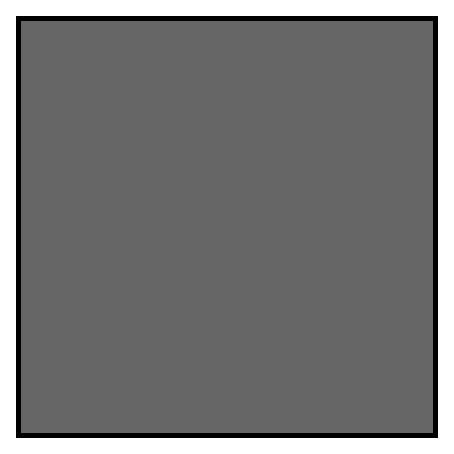
\includegraphics{example.eps}
% % figure caption is below the figure
% \caption{Please write your figure caption here}
% \label{fig:1}       % Give a unique label
% \end{figure}


% % ------ Methodology ------

% \section{Methodology}

% In this section, we will provide an intuitive and detailed explanation of MSAD-E. We will start with a description of the general pipeline, and then we will move to introducing the individual components from start to end.

% \subsection{Methodology}

% There is certain terminology that should be discussed prior to the pipeline. Firstly, a Model Selector (MS) is a time series classifier, e.g. a k-Nearest Neighbors (kNN) classifier, a Convolutional Neural Network (CNN), etc. Then, we have anomaly detectors (or detectors for short) which are (as the name suggests) the models for performing anomaly detection in time series. 

% Initially, time series are segmented into windows and fed to a trained MS. The MS outputs detector probabilities for each time series. Usually, while doing classification, we would do an argmax operation over these probabilities and select one detector as the prediction of the classifier. However, in our work, we use multiple predictions. So, after having the probabilities, we run multiple detectors over the time series and multiply by their predicted probabilities to get the weighted average ensemble. The produced anomaly score is a weighted combination of multiple anomaly scores. 

% \subsection{Analysis on averaging the top k detectors}
% In this subsection, we will dive deeper into the results of weighted averaging the top predictions of an MS. We will compare the different detectors and the different methods to get the results. We will compare weighted averaging with our previous approach, that is, predicting and using a single detector. Finally, we will evaluate whether the result is worth the overhead. The following subsection is organized into questions that we will pose, and we will answer in our effort to provide as much insight as possible from our findings.

% However, before we jump into the results, we will explain the setting of our experiment. From our previous work we select our best MS, namely \textbf{ConvNet-128}, \textbf{ResNet-1024}, \textbf{SiT-512}, and \textbf{kNN-1024} (the first part of each name refers to the architecture and the second part to the size of the input). The Rocket MS were not included into the analysis since the showcased very unstable behavior. These MS will be compared subsequently.

% Additionally, for each MS, there are two different methods for combining the probabilities between the windows of a time series. These methods are a) \textbf{Vote}, b) \textbf{Average}, and they will also be compared following. 

% Last but not least, our experiments exhibit, time series from around 16 different datasets to provide both robust results. Also, the number of Anomaly Detectors combined ranges from k = 1 (the case of using a single detector, not averaging), to k = 12 (the case of weighted averaging all detectors).

% \subsubsection{Is weighted averaging better, in terms of accuracy, than predicting and using a single anomaly detector?}
% Quick answer, yes... although things are rarely so simple. Our results show that overall there is an increase in AUC-PR when combining detectors. More precisely, combining 2 detectors (k = 2), already provides an increase of around 3-5\% which plateaus after 4 or 5 steps for k. This means that we don't have to combine all available detectors to get the best possible results. More precisely:

% \begin{table*}[t]
% \caption{AUC-PR Percentage Change for Different Models, Combine Methods, and k Values}
% \label{tab:AUC-PR-Percentage-Change}
% \begin{tabular}{llllllllllllll}
% \hline\noalign{\smallskip}
% Model Selector & Combine Method & \multicolumn{12}{c}{k} \\
% \cline{3-14} 
%  &  & 1 & 2 & 3 & 4 & 5 & 6 & 7 & 8 & 9 & 10 & 11 & 12 \\
% \noalign{\smallskip}\hline\noalign{\smallskip}
% \multirow{2}{*}{convnet128} & average & (0.48, 0.0) & (0.5, 5.19) & (0.51, 7.14) & \textbf{(0.52, 7.95)} & (0.52, 7.92) & (0.52, 7.76) & (0.51, 7.2) & (0.51, 6.65) & (0.51, 6.62) & (0.51, 6.65) & (0.51, 6.6) & (0.51, 6.59) \\
%  & vote & (0.48, 0.0) & (0.5, 5.5) & (0.51, 7.0) & (0.51, 7.78) & \textbf{(0.51, 8.14)} & (0.51, 8.12) & (0.51, 7.99) & (0.51, 8.0) & (0.51, 7.96) & (0.51, 7.98) & (0.51, 7.99) & (0.51, 7.98) \\
% \multirow{2}{*}{knn1024} & average & (0.34, 0.0) & (0.37, 8.51) & (0.38, 11.94) & (0.39, 13.7) & (0.4, 17.12) & (0.4, 18.63) & (0.41, 19.96) & (0.41, 20.6) & \textbf{(0.41, 20.61)} & (0.41, 20.54) & (0.41, 20.53) & (0.41, 20.54) \\
%  & vote & (0.35, 0.0) & (0.39, 10.49) & (0.39, 12.24) & (0.4, 12.9) & (0.4, 13.46) & (0.4, 13.56) & (0.4, 13.53) & \textbf{(0.4, 13.59)} & (0.4, 13.56) & (0.4, 13.56) & (0.4, 13.55) & (0.4, 13.55) \\
% \multirow{2}{*}{resnet1024} & average & (0.48, 0.0) & (0.49, 2.85) & (0.49, 3.36) & (0.5, 4.7) & (0.5, 5.49) & (0.5, 5.3) & (0.5, 5.42) & (0.5, 5.33) & \textbf{(0.5, 5.74)} & (0.5, 5.5) & (0.5, 5.72) & (0.5, 5.71) \\
%  & vote & (0.47, 0.0) & (0.48, 2.94) & (0.49, 3.93) & \textbf{(0.49, 4.07)} & (0.49, 4.0) & \textbf{(0.49, 4.07)} & (0.49, 4.05) & (0.49, 4.05) & (0.49, 4.05) & (0.49, 4.05) & (0.49, 4.05) & (0.49, 4.05) \\
% \multirow{2}{*}{sit512} & average & (0.48, 0.0) & (0.5, 3.21) & (0.5, 3.32) & (0.51, 5.09) & \textbf{(0.51, 5.44)} & (0.51, 5.08) & (0.51, 4.56) & (0.51, 4.49) & (0.51, 4.49) & (0.51, 4.46) & (0.51, 4.52) & (0.51, 4.52) \\
%  & vote & (0.48, 0.0) & (0.5, 3.1) & (0.5, 4.78) & (0.51, 5.52) & \textbf{(0.51, 5.77)} & (0.51, 5.73) & (0.51, 5.7) & (0.51, 5.71) & (0.51, 5.69) & (0.51, 5.69) & (0.51, 5.69) & (0.51, 5.69) \\
% \hline
% \end{tabular}
% \end{table*}






% \subsubsection{For which time series does it work better and why?}


% \subsubsection{Does any MS outperform the others? If yes, how?}


% \subsubsection{Which windows' probabilities combination method is better 'vote' or 'average'?}


% \subsubsection{Is there a plateau at some k or not? Is the behavior the same a) per time series, b) per dataset, and c) globally?}


% \subsubsection{What's the improvement to overhead trade-off? Do you think it is worth it, and in which cases?}


% \subsection{Analysis on combining anomaly detectors in general}




% %
% % For two-column wide figures use
% \begin{figure*}
% % Use the relevant command to insert your figure file.
% % For example, with the graphicx package use
%   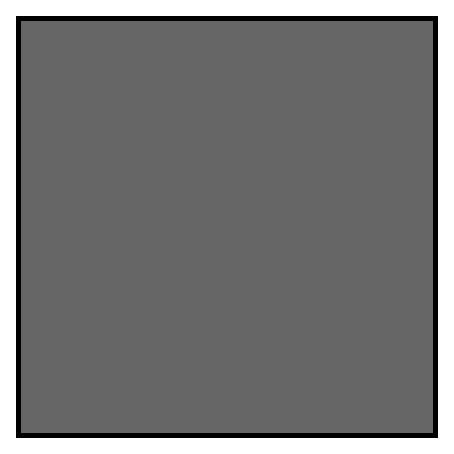
\includegraphics[width=0.75\textwidth]{example.eps}
% % figure caption is below the figure
% \caption{Please write your figure caption here}
% \label{fig:2}       % Give a unique label
% \end{figure*}
% %
% % For tables use
% \begin{table}
% % table caption is above the table
% \caption{Please write your table caption here}
% \label{tab:1}       % Give a unique label
% % For LaTeX tables use
% \begin{tabular}{lll}
% \hline\noalign{\smallskip}
% first & second & third  \\
% \noalign{\smallskip}\hline\noalign{\smallskip}
% number & number & number \\
% number & number & number \\
% \noalign{\smallskip}\hline
% \end{tabular}
% \end{table}


% \begin{acknowledgements}
% I would like to thank my mother and my father that support me in this great journey of my academic pursuits.
% \end{acknowledgements}

% BibTeX users please use one of
% \bibliographystyle{spbasic}      % basic style, author-year citations
\bibliographystyle{spmpsci}      % mathematics and physical sciences
% \bibliographystyle{spphys}       % APS-like style for physics
\bibliography{aaai22.bib}   % name your BibTeX data base

% Non-BibTeX users please use
% \begin{thebibliography}{}
% %
% % and use \bibitem to create references. Consult the Instructions
% % for authors for reference list style.
% %
% \bibitem{RefJ}
% % Format for Journal Reference
% Author, Article title, Journal, Volume, page numbers (year)
% % Format for books
% \bibitem{RefB}
% Author, Book title, page numbers. Publisher, place (year)
% % etc
% \end{thebibliography}

\end{document}
% end of file template.tex

